\documentclass[11pt]{article}

% Paquete para configurar márgenes y espaciado
\usepackage[a4paper, margin=2.5cm]{geometry}

% Paquete para el manejo de idiomas y codificación de fuentes
\usepackage[spanish]{babel}
\usepackage[utf8]{inputenc}
\usepackage[T1]{fontenc}

% Configuración de fuentes
\usepackage{mathptmx} % Times New Roman
\renewcommand{\rmdefault}{ptm}

% Configuración de títulos
\usepackage{titlesec}
\titleformat*{\section}{\fontsize{16}{18}\bfseries}
\titleformat*{\subsection}{\fontsize{14}{16}\bfseries}
\titleformat*{\subsubsection}{\fontsize{14}{16}\bfseries}

% Configuracion de bibliografia
\usepackage{fvextra}
\usepackage{csquotes}

\usepackage{biblatex} %Imports biblatex package
\addbibresource{resources/bibliography.bib} %Import the bibliography file

% Configuración de interlineado
\usepackage{setspace}
\onehalfspacing

% Configuración de encabezado y pie de página
\usepackage{fancyhdr}
\pagestyle{fancy}
\fancyhf{}
\chead{Análisis de lenguajes para sistemas concurrentes}
\rfoot{\thepage}
\lfoot{Civini, Foppiano, Mastricchio, Zulaica}

% Configuracion para que las imagenes no floten a otras secciones / sub-secciones

\usepackage{placeins}

\let\Oldsection\section
\renewcommand{\section}{\FloatBarrier\Oldsection}

\let\Oldsubsection\subsection
\renewcommand{\subsection}{\FloatBarrier\Oldsubsection}

\let\Oldsubsubsection\subsubsection
\renewcommand{\subsubsection}{\FloatBarrier\Oldsubsubsection}

% Configuración de espacio antes y después de los párrafos
\setlength{\parskip}{0pt}
\setlength{\parindent}{2em}
\setlength{\headheight}{13.6pt}

\usepackage{graphicx}
\usepackage{listings}

\PassOptionsToPackage{hyphens}{url}
\usepackage[colorlinks = true,
            linkcolor = blue,
            urlcolor  = blue,
            citecolor = blue,
            anchorcolor = blue]{hyperref}
\usepackage[dvipsnames]{xcolor}
\usepackage[newfloat]{minted}
\usepackage{cleveref}

\usemintedstyle{default}
\definecolor{bg}{RGB}{248,248,248}
% \definecolor{bg}{HTML}{282828}

\usepackage{caption}

\newenvironment{code}{\captionsetup{type=listing}}{}
\SetupFloatingEnvironment{listing}{name=Código}

\usepackage{float}

\newcommand{\badMetric}[1]{{\color{BrickRed}#1}}

\newcommand{\goodMetric}[1]{{\textbf{#1}}}

\usepackage{multirow}
\usepackage{multicol}

\renewcommand{\arraystretch}{1.4}

\usepackage{plantuml}
\usepackage{amsfonts} 
\usepackage{subcaption}

% Set figure/code/table numbering per section
\counterwithin{figure}{section}
\counterwithin{table}{section}
\counterwithin{listing}{section}



\setpythontexlistingenv{pythontexlisting}
\begin{document}

\tableofcontents
\newpage

\section{Resumen}

\section{Introducción}

\section{Contexto}

\subsection{Planificación}

\subsection{Entornos de despliegue} \label{sec:deploy_envs}

Se obtuvo acceso a 2 (dos) supercomputadoras de la Universidad de Córdoba (Facultad de Matemática, Astronomía, Física y Computación - FaMAF y del Centro de Cómputo de Alto Desempeño - CCAD), gracias a la colaboración de Rosa Wachenchauzer y Nicolás Wolovick. De aquí en adelante, llamaremos FaMAF-1 y FaMAF-2 a cada una de ellas:
\begin{itemize}
    \item FaMAF-1: procesador AMD EPYC 7643, 128 GB de memoria RAM, disco SSD de 894 GB.
    \item FaMAF-2: procesador E5-2680v4, 128 GB de memoria RAM, disco SSD de 223 GB.
\end{itemize}

\section{Introducción de Lenguajes}

\subsection{C++}

Es un lenguaje de referencia, estándar en la industria, versátil y poderoso. Más antiguo y de más bajo nivel que el resto de los lenguajes seleccionados. Siendo los aspectos destacados de su diseño el \textbf{rendimiento}, la \textbf{eficiencia} y la \textbf{flexibilidad de uso}.

Es un lenguaje compilado, sin administrador de paquetes o dependencias. No provee abstracciones nativas para la concurrencia, se utilizan threads o procesos.

Expectativas: Engorroso de utilizar debido al bajo nivel. Muy buen rendimiento.

\subsection{Scala}

Es un lenguaje que combina la programación orientada a objetos con la funcional. Está diseñado para ser \textbf{expresivo} (proveyendo abstracciones de alto nivel que aumentan la productividad y simplifican el código), \textbf{escalable} (adaptándose a entornos concurrentes y distribuidos, priorizando la interoperabilidad) y \textbf{seguro} (incluyendo chequeos estáticos y estructuras thread-safe).

Corre sobre la \textbf{JVM}, pudiendo hacer uso de muchos recursos del ecosistema de Java. Implementa \textbf{Futures} como unidad para tareas concurrentes.

Expectativas: Fácil de aprender y utilizar. Rico en recursos externos. Rendimiento acotado por el uso de máquina virtual.

\subsection{Go}

Un lenguaje moderno que toma prestadas ideas de otros. Es \textbf{expresivo}, \textbf{conciso}, \textbf{limpio} y \textbf{eficiente}; destacando por la facilidad de aprenderlo y sus herramientas nativas para la \textbf{concurrencia}.

Corre sobre un runtime que se encarga del manejo de memoria. Implementa \textbf{goroutines} como threads livianos.

Expectativas: Fácil de aprender. Buen rendimiento.

\subsection{Julia}

Es un lenguaje orientado a la ciencia de datos. Busca ser \textbf{dinámico}, \textbf{flexible} y \textbf{eficiente}.

Corre sobre un runtime propio. Soporta concurrencia basada en \textbf{tareas}.

Expectativas: Fácil de aprender pero no necesariamente provee herramientas de uso general. Rendimiento variable al caso.

\subsection{Elixir}

Un lenguaje funcional basado en el paradigma de \textbf{actores}. Pensado para el desarrollo de aplicaciones \textbf{escalables} y \textbf{mantenibles}.

Corre por encima de la VM de Erlang, conocida por el desarrollo de sistemas distribuidos de baja latencia y tolerantes a fallos. El modelo de actores es concurrente por naturaleza.

Expectativas: Difícil de aprender y utilizar debido al cambio de paradigma. Buena performance para sistemas distribuidos, variable para otros casos.

\subsection{Python}

TBA

\subsection{Rust}

TBA

\subsection{Zig}

TBA

\subsection{Ruby}

TBA


\subsection{Java}

TBA

\newpage

\section{Área: Sistemas Distribuidos}

Definimos un sistema distribuido como una colección de computadoras independientes, que se comunican para cumplir un objetivo común.

Este tipo de sistemas es de gran relevancia en la actualidad, donde los volúmenes de datos son cada vez mayores \cite{sis_dist:data_volume}, mientras que el costo de cómputo paralelo es cada vez menor \cite{sis_dist:compute_price}.

Los desafíos que enfrenta un sistema distribuido son muchos

\begin{itemize}
    \item Comunicación: en muchos casos, los procesos solo pueden intercambiar información a través de Internet. Por lo tanto, la comunicación se da a través de paquetes TCP/UDP y, en consecuencia, toda la información debe serializarse y adaptarse a ese modelo
    \item Sincronización: los procesos deben estar debidamente coordinados para poder cumplir satisfactoriamente sus objetivos. Para esto se desarrollaron numerosos algoritmos: de consenso (Paxos \cite{sis_dist:paxos}, Raft \cite{sis_dist:raft}) y de elección de líder (Bully \cite{sis_dist:bully})
    \item Tolerancia a fallos: al aumentar el número de componentes involucrados en un sistema distribuido, la probabilidad de que al menos uno falle aumenta. Esto puede verse fácilmente con un ejemplo simplificado.
    
    Sean $X_1, X_2, \dots, X_n$ un conjunto independiente de componentes, y sea $F_i$ el evento ``El componentes $X_i$ sufre un fallo''. Suponiendo que todos los componentes tienen la misma probabilidad de fallar ($\mathbb{P}(F_i)=p$, con $0<p\leq1$), entonces la probabilidad de que al menos uno de ellos falle se puede calcular como

    \begin{equation}
        1 - \mathbb{P}(\bigcap_{i=0}^n F_i) = 1 - \prod_{i=1}^n \mathbb{P}(F_i) = 1 - p^n
    \end{equation}

    Esta propiedad pone en evidencia la necesidad de los sistemas distribuidos de manejar, de una u otra forma, los errores. Una de los técnicas más utilizadas es la tolerancia a fallos, que se define como el método para mantener los sistemas interconectados, manteniendo su fiabilidad y disponibilidad \cite{sis_dist:fault_tol}
\end{itemize}

La elección de un lenguaje de programación puede atenuar o amplificar estos retos, por lo que un análisis de los mismos puede resultar muy beneficioso. Algunos lenguajes, como C, fueron creados en un contexto histórico previo a los sistemas distribuidos. Como consecuencia, las herramientas que proveen pueden resultar un poco primitivas para la tarea. Otros más modernos, como Julia, se diseñaron poniendo el foco en la computación distribuida.

Para este tipo de sistemas nos interesa evaluar el modelo de concurrencia \textit{multi-computing}. En éste, los componentes son computadoras comunicadas a través de la red.

\subsection{Casos de uso}

Dentro del área de estudio, desarrollamos 2 (dos) casos de uso, poniendo el foco en sistemas de procesamiento de datos

\subsubsection{Grid Search Distribuido}

La optimización de funciones es un problema clásico con infinidad de aplicaciones. Cuando algo puede modelarse con una función, generalmente estamos interesados en obtener los valores máximos y míninmos que toma, junto con los valores de \textit{input} que los generan. A lo largo del tiempo se desarrollaron diferentes métodos para resolver este problema, algunos analíticos, como los multiplicadores de Lagrange \cite{sis_dist:lagrange}; y otros numéricos, como el método Simplex \cite{sis_dist:simplex}. La \textbf{búsqueda en grilla} es uno de ellos.

Teniendo una función que recibe `n' parámetros numéricos, podemos definir un rango (es decir, un valor mínimo y uno máximo) y un paso (que será la distancia entre los puntos) para cada parámetro y definir una grilla de puntos en `n' dimensiones.
Cada dimensión de la grilla corresponde a un parámetro y cada punto es una configuración definida de los valores de esos parámetros.
La función se evalúa en cada punto de dicha grilla.

Se plantea un sistema distribuido para la evaluación de una función arbitraria en un rango determinado de parámetros que se ejecutará en nodos trabajadores.

Se utiliza una arquitectura común para cada desarrollo, compuesta por un nodo \textit{manager} que define y particiona el trabajo, así como un conjunto de trabajadores (\textit{workers}) para procesarlo. La comunicación de estos será entre colas, o mecanismos similares. Ver figura \ref{fig:sis_dist:grid_search_arch}.

\begin{figure}[h]
    \centering
    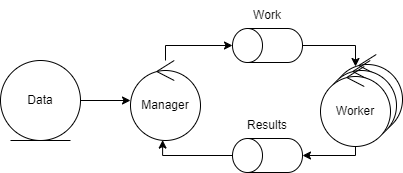
\includegraphics[scale=0.5]{resources/distributed_systems/grid_search_arch.png}
    \caption{Arquitectura de Grid Search}
    \label{fig:sis_dist:grid_search_arch}
\end{figure}

\subsubsection{Pipeline Procesamiento de Imágenes}

En los últimos años, las redes neuronales profundas ganaron mucha popularidad gracias a su capacidad para resolver problemas reales complejos \cite{sis_dist:dnn}. Un conjunto de redes muy prometedor es el de las redes neuronales convolucionales, ampliamente utilizadas para el análisis de imágenes \cite{sis_dist:cnn}. Estas redes, por lo general, requieren un \textit{input} normalizado, es decir, imágenes en un determinado formato, tamaño, etc. Como los datasets pueden llegar a ser muy grandes, puede ser beneficioso implementar este proceso de manera distribuida, a través de un pipeline de procesamiento.

Se plantea un sistema donde cada etapa realiza una transformación específica
\begin{itemize}
    \item Formato: Conversión al formato PNG\cite{sis_dist:png}
    \item Resolución: Reducción a una resolución de 100x100 pixeles
    \item Tamaño: Recortado del cuadrado central de 30x30 pixeles
\end{itemize}

En la Figura \ref{fig:sis_dist:ip_example} se puede observar un ejemplo de cada una de estas etapas.

\begin{figure}
    \centering
    \begin{subfigure}[b]{0.3\textwidth}
        \centering
        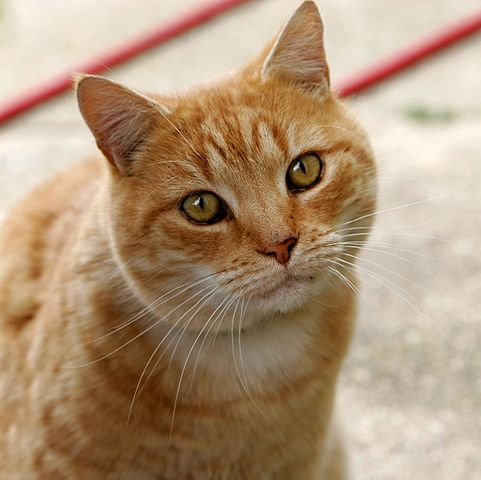
\includegraphics[width=\textwidth]{resources/distributed_systems/pipeline_images/input.jpg}
        \caption{Original}
    \end{subfigure}
    \hspace{10mm}
    \begin{subfigure}[b]{0.3\textwidth}
        \centering
        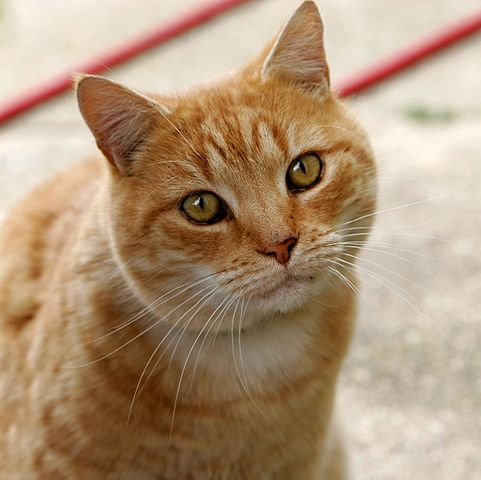
\includegraphics[width=\textwidth]{resources/distributed_systems/pipeline_images/formatted.png}
        \caption{Convertida a PNG}
    \end{subfigure}
    
    \begin{subfigure}[b]{0.3\textwidth}
        \centering
        
\includegraphics[width=\textwidth]{resources/distributed_systems/pipeline_images/scaled.png}
        \caption{Reducida a 100x100 pixeles}
    \end{subfigure}
    \hspace{10mm}
    \begin{subfigure}[b]{0.3\textwidth}
        \centering
        
\includegraphics[width=\textwidth]{resources/distributed_systems/pipeline_images/cropped.png}
        \caption{Recortada a 30x30 pixeles}
    \end{subfigure}
    \caption{Ejemplo de transformaciones del pipeline de procesamiento de imágenes}
    \label{fig:sis_dist:ip_example}
\end{figure}

La arquitectura está compuesta por un nodo Manager y etapas de trabajadores para cada transformación. El trabajo es distribuido mediante colas, o herramientas similares. Las imágenes en sí son accedidas mediante un sistema de archivos compartido. Ver figura \ref{fig:sis_dist:image_processing_arch}.

\begin{figure}[h]
    \centering
    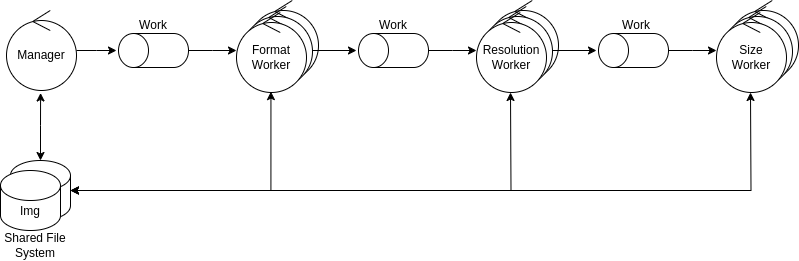
\includegraphics[scale=0.5]{resources/distributed_systems/image_processing_arch.png}
    \caption{Arquitectura de Procesamiento de Imágenes}
    \label{fig:sis_dist:image_processing_arch}
\end{figure}

\subsection{Despliegue}

En esta sección se especifican los detalles de despliegue. Esto incluye los entornos de ejecución y datos utilizados.

\subsubsection{Entornos}

Debido a que FaMAF-1 se encontraba en uso durante el período de benchmarking, los casos fueron ejecutados solamente en FaMAF-2 (Ver sección \ref{sec:deploy_envs}). De esta manera, nos aseguramos de que las métricas tengan la menor interferencia posible con otros programas.

Además, se realizaron ejecuciones complementarias en Google Cloud Platform (GCP), a modo de obtener mediciones comparativas en diferentes entornos. En particular, las máquinas virtuales utilizadas cuentan, para la versión n1, con procesador Intel Cascade Lake y Ice Lake (sujeto a disponibilidad), 2 vCPU (un único hardware thread), 8 GB de memoria RAM, disco SSD local; para la versión n2, cuentan con procesador Intel Skylake, Broadwell, Haswell, Sandy Bridge, y Ivy Bridge, 1 vCPU (un unico hardware thread), $3.75$ GB de memoria RAM, disco SSD local\footnote{Para más información, el ambiente completo se encuentra detallado en formato de archivos de Terraform, disponible en \url{https://github.com/tpf-concurrent-benchmarks/gcp_deployment}}.

\subsubsection{Dataset}

Para la evaluación del grid-search: se ejecutará la función Griewank \cite{sis_dist:griewank} dentro del rango \break
[-600; 600; $0.2$]\^{}3, es decir, el rango que va de -600 a 600 con paso de $0.2$ en 3 parámetros. Utilizando un máximo de 10800000 números por paquete, limitando el tamaño de los rangos que reciben los trabajadores por tarea. Buscando la configuración de parámetros que devuelven el mínimo resultado.

Para la evaluación del procesamiento de imágenes: Las imágenes se transforman a formato png, se escalan a una resolución de 100x100 y se recortan los 30x30 px centrales. Se utiliza en dataset: BIRDS 525 SPECIES \cite{sis_dist:birds_dataset} aumentado: espejando horizontalmente y verticalmente las imágenes \footnote{El script utilizado puede encontrarse en: \url{https://github.com/tpf-concurrent-benchmarks/various/blob/main/image_processing/image_multiplicator.py}. No se utilizaron las rotaciones.}.

\subsection{Implementación}

En esta sección se desarrollan los detalles de implementación para cada lenguaje. Se incluyen diagramas con fin de explicar las particularidades de cada arquitectura. Así como secciones de código que sean útiles para transmitir las características y utilización de los lenguajes y sus \textit{frameworks}.

\subsubsection{C++}

Se seleccionó este lenguaje como \textit{baseline} de comparación con otros lenguajes, ya que es un lenguaje clásico y de uso general que se utiliza en varias soluciones distribuidas \cite{cpp:ex:ray-io} \cite{cpp:ex:red-panda}.

Para la comunicación de procesos se utilizó \textbf{ZMQ} \cite{cpp:lib:zmq}, el cual provee colas de mensajería ligeras y adecuadas para este trabajo.

En cuanto a la implementación, se aprovecharon al máximo las capacidades que ofrece C++ al ser un lenguaje de programación de \textbf{bajo nivel}. La capacidad de asignar memoria manualmente, crear estructuras de datos compactas y eficientes y el uso de  templates, permitió desarrollar una aplicación sumamente eficiente para este caso.

Adicionalmente, gracias a que ZMQ no hace uso de una instancia dedicada de \textit{middleware} también se redujo mucho el costo adicional en comunicación.

En el caso del procesamiento de imágenes, al haber utilizado ZMQ, nos requirió de crear procesos que actúan como un \textit{broker}, como se puede ver en la Figura \ref{fig:cpp:image_processing_arch}. Es decir, procesos que actúan como intermediarios que permiten recibir mensajes de N procesos, y al mismo tiempo, enviar mensajes a N procesos bajo algún algoritmo (por ejemplo, \textit{round-robin}).

\begin{figure}[ht]
    \centering
    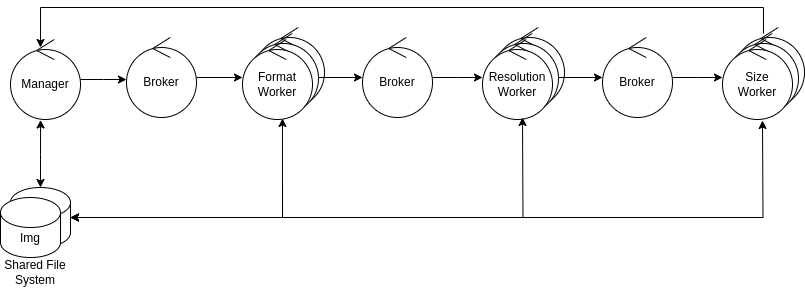
\includegraphics[scale=0.4]{resources/distributed_systems/cpp/image_processing_arch.png}
    \caption{Arquitectura de Procesamiento de Imágenes en C++}
    \label{fig:cpp:image_processing_arch}
\end{figure}

Estos procesos \textit{broker} se limitan a recibir los mensajes de una etapa de \textit{workers} y enviarlos a la siguiente, como podemos ver en el Código \ref{code:cpp:broker}.

\begin{listing}[ht]
\begin{minted}[bgcolor=bg, breaklines]{c++}
int main()
{
    Protocol protocol(getPushPort(), getPullPort());
    bool shouldStop = false;

    while (!shouldStop)
    {
        std::string message = protocol.receive();
        if (message == Constants::STOP_MESSAGE)
        {
            shouldStop = true;
            continue;
        }
        protocol.send(message);
    }
    protocol.close();
}
\end{minted}
\caption{Función principal de un \textit{broker} genérico en C++}
\label{code:cpp:broker}
\end{listing}

Por otro lado, el funcionamiento de los trabajadores es independiente de quién recibe los mensajes, la lógica de comunicación está abstraída de su función y es configurada por separado. Podemos ver el funcionamiento de uno de los \textit{workers} en el Código \ref{code:cpp:format_worker}.

\begin{listing}[ht]
\begin{minted}[bgcolor=bg, breaklines]{c++}
while (!shouldStop)
{
    std::string message = protocol.receive();
    if (message == Constants::STOP_MESSAGE)
    {
        shouldStop = true;
    }
    else
    {
        std::string imageName = message.substr(message.find_last_of('/') + 1);
        std::string newImageName = imageName.substr(0, imageName.find_last_of('.')) + ".png";

        std::chrono::milliseconds start_time_ms = std::chrono::duration_cast<std::chrono::milliseconds>(
            std::chrono::system_clock::now().time_since_epoch());

        change_format(message, "../../shared_vol/formatted/" + newImageName);

        std::chrono::milliseconds end_time_ms = std::chrono::duration_cast<std::chrono::milliseconds>(
            std::chrono::system_clock::now().time_since_epoch());
        std::chrono::milliseconds completion_time = end_time_ms - start_time_ms;
        statsdClient.timing("work_time", completion_time.count(), 1);
        statsdClient.increment("results_produced");

        protocol.send("../../shared_vol/formatted/" + newImageName);
    }
}
\end{minted}
\caption{Extracto de la función principal de un \textit{format worker} en C++}
\label{code:cpp:format_worker}
\end{listing}

Adicionalmente, se debió implementar polling sobre dos tipos sockets en simultáneo (ver Codigo \ref{code:cpp:polling}). Se utiliza un socket push-pull para el envío de tareas, este funciona repartiendo las tareas equitativamente. Y se utiliza un socket pub-sub para los mensajes al finalizar el procesamiento.

\begin{listing}[ht]
\begin{minted}[bgcolor=bg, breaklines]{c++}
std::string Protocol::receive()
{
    zmq::pollitem_t items[] = {
            {receiver_, 0, ZMQ_POLLIN, 0},
            {end_work_, 0, ZMQ_POLLIN, 0}};
    zmq::poll(&items[0], 2, -1);

    if (items[0].revents & ZMQ_POLLIN)
    {
        zmq::message_t message;
        const zmq::recv_result_t &anOptional = receiver_.recv(message);
        if (!anOptional.has_value())
        {
            return "Error message";
        }
        return std::string(static_cast<char *>(message.data()), message.size());
    }
    else if (items[1].revents & ZMQ_POLLIN)
    {
        zmq::message_t message;
        const zmq::recv_result_t &anOptional = end_work_.recv(message);
        if (!anOptional.has_value())
        {
            return "Error message";
        }
        return std::string(static_cast<char *>(message.data()), message.size());
    }
    else
    {
        return "Error message";
    }
}
\end{minted}
\caption{Extracto de la función principal de un \textit{format worker} en C++}
\label{code:cpp:polling}
\end{listing}

\subsubsection{Scala}

Se seleccionó este lenguaje porque es utilizado para el desarrollo de herramientas de procesamiento distribuido populares, como Apache Spark \cite{scala:ex:spark}; reflejando el estándar de la industria para esta área.

Se utilizó \textbf{RabbitMQ} \cite{scala:lib:rabbit} como \textit{middleware} para la distribución de trabajo. Este \textit{middleware} tiene la particularidad de requerir un \textit{broker} centralizado en el cual se definirán las colas de comunicación. Podemos ver en la Figura \ref{fig:scala:image_processing_arch} la arquitectura del \textit{pipeline} de imágenes, donde se aprecia que las conexiones de todos los componentes son con el \textit{broker} de RabbitMQ. El flujo de datos y la arquitectura es igual a los definidos en la figura \ref{fig:sis_dist:image_processing_arch}, pero el manejo de todas las colas es mediante este \textit{broker}.

\begin{figure}[ht]
    \centering
    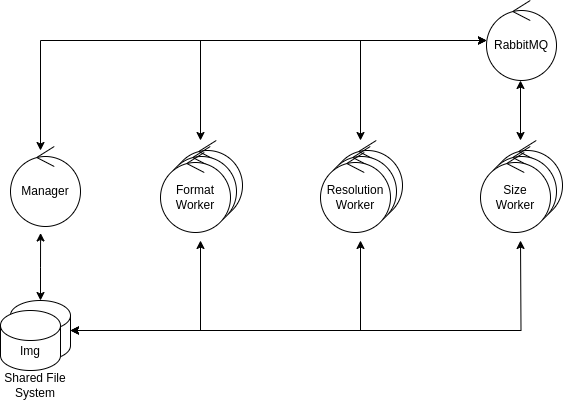
\includegraphics[scale=0.4]{resources/distributed_systems/scala/image_processing_arch.png}
    \caption{Arquitectura de Procesamiento de Imágenes en Scala}
    \label{fig:scala:image_processing_arch}
\end{figure}

Se intentó utilizar \textbf{Akka} \cite{scala:lib:akka}, un \textit{framework} popular para sistemas distribuidos basado en actores, pero su uso resultó ser dificultoso y se descartó en pos de mantener el cronograma.

Se aprovecharon ampliamente las herramientas del lenguaje para evaluación \textbf{\textit{lazy}} de iteradores. Podemos ver en el Código \ref{code:scala:split} el método que genera las particiones de trabajo de manera \textit{lazy} para la búsqueda en grilla.

\begin{listing}[ht]
\begin{minted}[bgcolor=bg, breaklines]{scala}
def split(maxChunkSize: Int, precision: Option[Int] = None): Iterator[Work] = {
    val minBatches = Math.ceil(size.toDouble / maxChunkSize)
    val partitionsPerInterval = calcPartitionsPerInterval(minBatches.toInt)


    val listOfIterator = for (intervalPos <- intervals.indices) yield {
        val iterator = intervals(intervalPos).split(partitionsPerInterval(intervalPos), precision)
        CircularIterator(iterator, partitionsPerInterval(intervalPos), precision)
    }

    WorkPlan(listOfIterator.toList,aggregator).iterator
}
\end{minted}
\caption{Fragmento de métodos de particionamiento de trabajo en Scala}
\label{code:scala:split}
\end{listing}

Otra herramienta que se aprovechó fue el uso de \textit{Traits}, que permiten abstraer lógica común. En el Código \ref{code:scala:basic_transformer} podemos ver el Trait `BasicTransformer' que encapsula la lógica de comunicación que utilizaran todos los workers del pipeline de procesamiento de imágenes.

\begin{listing}[ht]
\begin{minted}[bgcolor=bg, breaklines]{scala}
trait BasicTransformer {
    val inputQueue: String
    val outputQueue: String
    val endEvent: String
    type InputType
    type OutputType
    implicit val reader: Reader[InputType]
    implicit val writer: Writer[OutputType]

    def transform(input: InputType): Option[OutputType]

    private def setUpConsumer(middleware: MessageQueue): Unit = {
        middleware.setConsumer(inputQueue, input => {
            val convertedInput = read[InputType](input)

            val output = transform(convertedInput)
            output.foreach(o => {
                val outputString = default.write(o)
                middleware.produce(outputQueue, outputString.getBytes("UTF-8"))
            })
            true
        })
    }

    def start(middleware: MessageQueue): Unit = {
        setUpConsumer(middleware)
        val stopPromise = Promise[Unit]()

        middleware.subscribe(endEvent, end => {
            println(s"Received end: ${new String(end, "UTF-8")}")
            stopPromise.success(())
            true
        })
        println("Starting to consume")
        middleware.startConsuming(Some(stopPromise.future))
        middleware.close()
    }
}
\end{minted}
\caption{Trait comun para \textit{workers} de imagen en Scala}
\label{code:scala:basic_transformer}
\end{listing}

En el Código \ref{code:scala:resolution_worker} podemos ver la implementación del \textit{resolution worker}, donde solo es necesaria la función de transformación de imagen y la lógica de comunicación, sincronización y \textit{logeo} están abstraídas.

\begin{listing}[ht]
\begin{minted}[bgcolor=bg, breaklines]{scala}
case class ResolutionWorker(inputQueue: String,
                            outputQueue: String,
                            endEvent: String,
                            targetWidth: Int,
                            targetHeight: Int) extends BasicTransformer {
    override type InputType = FileName
    override type OutputType = FileName

    override implicit val reader: default.Reader[InputType] = fileNameRW
    override implicit val writer: default.Writer[OutputType] = fileNameRW

    override def transform(input: InputType): Option[OutputType] = {
        val sourcePath = input.path
        val sourceName = input.name
        val sourceFileName = s"$sourcePath/$sourceName"

        val targetPath = "./shared/scaled"
        val targetFileName = s"$targetPath/$sourceName"

        try {
            ImageUtils.scale(sourceFileName, targetFileName, targetWidth, targetHeight, ImageFormat.Png())
            Some(FileName(targetPath, sourceName))
        } catch {
            case e: java.io.FileNotFoundException =>
                println(s"Input file $sourceFileName not found - skipping")
                None
        }
    }
}
\end{minted}
\caption{Implementación de \textit{resolution worker} en Scala}
\label{code:scala:resolution_worker}
\end{listing}

\subsubsection{Go}

Sus aplicaciones en sistemas distribuidos son aún jóvenes, pero está tomando popularidad y generando proyectos interesantes \cite{go:ex:awesome-go}; lo cual lo convierte en un buen lenguaje para comparar.

Para la comunicación entre sistemas en Go se usó \textbf{NATS} \cite{go:lib:nats}, un \textit{middleware} orientado a los mensajes desarrollado en Go. Al igual que RabbitMQ hace uso de una instancia intermedia para la entrega de mensajes que provee persistencia, tolerancia a fallas y balanceo de cargas. Podemos ver la adaptación de la arquitectura del \textit{pipeline} de procesamiento de imágenes en la figura \ref{fig:go:image_processing_arch}

\begin{figure}[ht]
    \centering
    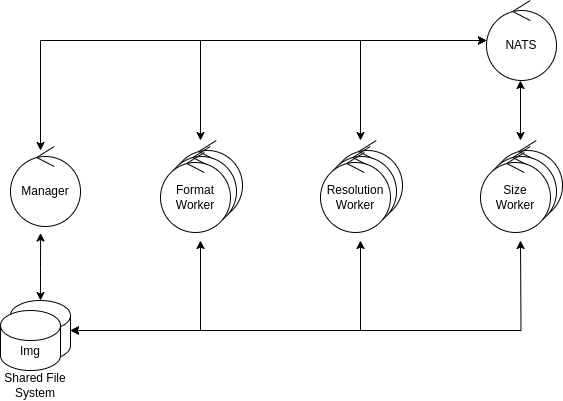
\includegraphics[scale=0.4]{resources/distributed_systems/go/image_processing_arch.png}
    \caption{Arquitectura de Procesamiento de Imágenes en Go}
    \label{fig:go:image_processing_arch}
\end{figure}

Dentro de NATS, se usó su modelo de publicador y suscriptor en el cual los trabajadores se suscriben a la cola para recibir el trabajo. Podemos ver en el Código \ref{code:go:size_worker} la lógica principal del trabajador de tamaño en el `pipeline' de imágenes, donde se realiza la suscripción a la cola de entrada y la definición del \textit{callback} al recibir un mensaje.

\begin{listing}[ht]
\begin{minted}[bgcolor=bg, breaklines]{go}
func subscribeForWork(conn *nats.Conn, workerConfig config.Config, statsdClient statsd.Statter) {
	_, err := conn.QueueSubscribe(workerConfig.Queues.Input, "workers_group", func(msg *nats.Msg) {
		imagePath := string(msg.Data)
		newImagePath := createOutputDir(imagePath)

		startTime := time.Now()

		image_processing.CropCentered(imagePath, newImagePath, workerConfig.Worker.TargetWidth, workerConfig.Worker.TargetHeight)

		endTime := time.Now()
		elapseTime := endTime.Sub(startTime).Milliseconds()
		err := statsdClient.Timing("work_time", elapseTime, 1.0)
		if err != nil {
			log.Fatalf("Error sending metric to statsd: %s", err)
		}

		err = statsdClient.Inc("results_produced", 1, 1.0)
		if err != nil {
			log.Fatalf("Error sending metric to statsd: %s", err)
		}

		err = conn.Publish(workerConfig.Queues.Output, []byte(common.JobDoneMessage))
		if err != nil {
			log.Fatalf("Error publishing to queue: %s", err)
		}
	})
	if err != nil {
		log.Fatalf("Error subscribing to queue: %s", err)
	}
}
\end{minted}
\caption{Fragmento de \textit{size worker} en Go}
\label{code:go:size_worker}
\end{listing}

Se usaron structs para representar los datos y se siguió un paradigma imperativo procedural para implementar el comportamiento. Podemos ver en el código \ref{code:go:grid_search} la implementación principal de los \textit{workers} de \textit{grid search}, donde la información es almacenada en el struct `GridSearch', cuyo metodo `Search' iterara la grilla y acumulara los resultados al ejecutar la funcion.

\begin{listing}[ht]
\begin{minted}[bgcolor=bg, breaklines]{go}
type GridSearch struct {
	params      *Params
	result      float64
	totalInputs uint64
	accumType   string
	input       [Size]float64
}

func (gs *GridSearch) Search(callback func([Size]float64) float64) {
	accumulator := NewAccumulator(gs.accumType)

	for i := int64(0); i < gs.params.getTotalIterations(); i++ {
		params := gs.params.getCurrent()
		result := callback(params)
		accumulator.Accumulate(result, params)
		gs.params.next()
	}
	gs.result = accumulator.GetResult()
	gs.input = accumulator.GetInput()
}
\end{minted}
\caption{Lógica principal de \textit{worker} de \textit{grid search} en Go}
\label{code:go:grid_search}
\end{listing}


\subsubsection{Julia}

Se seleccionó este lenguaje debido a que posee una \textbf{biblioteca nativa} para procesamiento distribuido \cite{jl:lib:distributed}, mostrando que es un área de interés del lenguaje.

El uso de esta biblioteca permite definir una arquitectura maestro-esclavo, donde los \textit{workers} se registran con el \textit{manager} y este es el encargado de distribuir y coordinar los procesos. Podemos ver en la figura \ref{fig:jl:image_processing_arch} la adaptación del \textit{pipeline} de procesamiento de imágenes, donde la comunicación entre procesos se da por medio del manager.

\begin{figure}[ht]
    \centering
    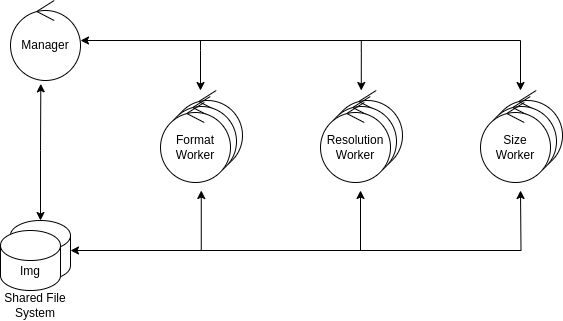
\includegraphics[scale=0.4]{resources/distributed_systems/jl/image_processing_arch.png}
    \caption{Arquitectura de Procesamiento de Imágenes en Julia}
    \label{fig:jl:image_processing_arch}
\end{figure}

En específico, para la implementación de \textbf{grid search} se empleó la capacidad de ejecutar un \textit{map} en un pool de \textit{workers}. El hecho de que estos \textit{workers} sean procesos distribuidos es transparente  para nosotros. Podemos ver en el Código \ref{code:jl:pmap} el empleo de `pmap' y el decorador `everywhere', que indica que secciones de código están definidas para todos los contextos (que serán aquellas que ejecutaran los \textit{workers}).

\begin{listing}[ht]
\begin{minted}[bgcolor=bg, breaklines]{julia}
@everywhere function evaluate_for_partition(sub_work_partition)
    map(sub_work_partition) do sub_work
        res = StatsLogger.runAndMeasure("work_time") do
            Works.evaluate_for!(sub_work, VALUES, RESULTS)
        end
        StatsLogger.increment("results_produced")
        return res
    end
end

function distribute_work(sub_works_parts, pool)
    @showprogress pmap(pool, sub_works_parts) do sub_work_partition
        evaluate_for_partition(sub_work_partition)
    end
end
\end{minted}
\caption{Distribución de tareas de \textit{grid search} en Julia}
\label{code:jl:pmap}
\end{listing}

Por otro lado, para el \textbf{procesamiento de imágenes} se emplearon `Canales Remotos' como colas de tareas, los cuales están definidos en el nodo `manager', haciendo que este funcione como `broker'.

Podemos ver en el Código \ref{code:jl:channels} la definición de estos canales. Y en el código \ref{code:jl:pipeline} la definición del \textit{pipeline}. De modo que tanto la arquitectura, los canales de comunicación y la funcionalidad de los trabajadores están definidos por código en el nodo `manager'.

\begin{listing}[ht]
\begin{minted}[bgcolor=bg, breaklines]{julia}
format_channel = RemoteChannel(()->Channel{String}(32))
resolution_channel = RemoteChannel(()->Channel{String}(32))
size_channel = RemoteChannel(()->Channel{String}(32))
result_channel = RemoteChannel(()->Channel{String}(32))

close_channels = () -> for chan in [format_channel, resolution_channel, size_channel, result_channel]
    close(chan)
end
get_channels() = format_channel, resolution_channel, size_channel, result_channel, close_channels
\end{minted}
\caption{Creación de canales remotos en Julia}
\label{code:jl:channels}
\end{listing}

\begin{listing}[ht]
\begin{minted}[bgcolor=bg, breaklines]{julia}
function start_worker_stage( workers::Array, handler::Function, in_channel::RemoteChannel, out_channel::RemoteChannel, type="worker" )
    for (i, p) in enumerate(workers)
        remote_do( worker_loop, p, handler, in_channel, out_channel, string(type, ".", i-1) )
    end
end

function start_pipeline()
    println("Starting workers")
    format_channel, resolution_channel, size_channel, result_channel = get_channels()
    format_workers, resolution_workers, size_workers = get_workers()

    # Start Format workers
    start_worker_stage( format_workers, format_handler, format_channel, resolution_channel, "format" )
    
    # Start Resolution workers
    start_worker_stage( resolution_workers, resolution_handler, resolution_channel, size_channel, "resolution" )
    
    # Start Size workers
    start_worker_stage( size_workers, size_handler, size_channel, result_channel, "size" )

    return format_channel, result_channel
end
\end{minted}
\caption{Definición del \textit{pipeline} de procesamiento de imágenes en Julia}
\label{code:jl:pipeline}
\end{listing}

\subsubsection{Elixir}

La VM de Erlang es muy utilizada para sistemas distribuidos \cite{elx:ex:companies} \cite{scala:lib:rabbit}. Elixir nos permite comparar ese entorno y su sistema de actores mediante una interfaz más moderna; lo cual nos llevó a seleccionar este lenguaje para comparar.

Se creó un \textbf{framework} de distribuidos basado en las herramientas de \textbf{actores distribuidos} nativas \footnote{Para más información, se desarrolla en la sección \ref{sec:anex:elixir_pipelines} o en la \href{https://github.com/tpf-concurrent-benchmarks/image_processing_elixir/blob/main/distributed_pipeline/lib/nodes/README.md}{documentación del código}} debido a que no se encontraron herramientas externas que cumplieran con las especificaciones que buscábamos.

Podemos ver en la figura \ref{fig:elx:image_processing_framework} la definición de procesos del \textit{pipeline} de imagenes utilizando el \textit{framework}. Se definen 4 tipos de nodo:
\begin{enumerate}
\item Fuente (\textit{Source}): Ingresa los datos al sistema, se los enviará a la primer etapa de workers.
    \item Trabajador (\textit{Worker}): Realiza el procesamiento, recibiendo datos de una fuente y enviándolas a un sumidero.
    \item   Mediador (\textit{Broker}): Hace de fuente y de sumidero, repartiendo tareas entre etapas de trabajadores.
    \item  Sumidero (\textit{Sink}): Recibe los resultados al final del \textit{pipeline}
\end{enumerate}

\begin{figure}[ht]
    \centering
    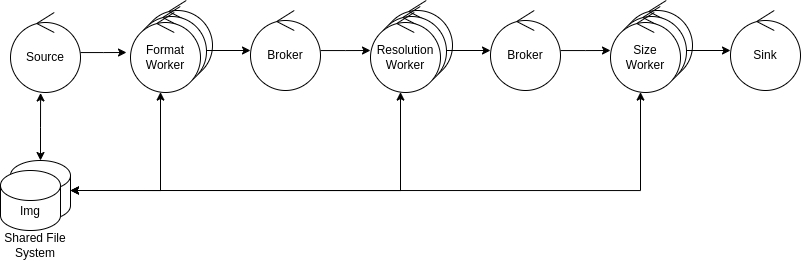
\includegraphics[scale=0.4]{resources/distributed_systems/elixir/image_processing_framework.png}
    \caption{Procesos de Procesamiento de Imágenes en Elixir}
    \label{fig:elx:image_processing_framework}
\end{figure}

Por otro lado, podemos ver en la figura \ref{fig:elx:image_processing_arch} el despliegue real del sistema, donde los procesos `source', `sink' y `broker' son ejecutados dentro del nodo `manager'

\begin{figure}[ht]
    \centering
    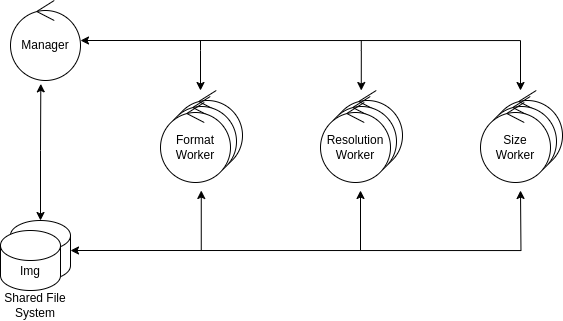
\includegraphics[scale=0.4]{resources/distributed_systems/elixir/image_processing_arch.png}
    \caption{Arquitectura de Procesamiento de Imágenes en Elixir}
    \label{fig:elx:image_processing_arch}
\end{figure}

Al igual que en Julia, el código está completamente definido sobre el nodo manager. Este es este quien asigna la funcionalidad de los trabajadores, además de proveerles el trabajo. Podemos observar la definición del sistema para \textit{grid search} en el código \ref{code:elx:gs} y para el \textit{pipeline} de imágenes en el código \ref{code:elx:ip}. El método `start\_link' es el que instancia los actores locales de `source', `sink' y `broker'; mientras que los trabajadores remotos son iniciados mediante `start\_remote\_worker'

\begin{listing}[ht]
\begin{minted}[bgcolor=bg, breaklines]{elixir}
def distributed_gs do
    config = ConfigReader.get_config("/app/lib/resources/data.json", :manager)
    IO.puts("Config read: #{inspect(config)}")
    data = Enum.at(config["data"], 0)
    data2 = Enum.at(config["data"], 1)
    data3 = Enum.at(config["data"], 2)
    interval = Interval.newInterval(Enum.at(data, 0), Enum.at(data, 1), Enum.at(data, 2))
    interval2 = Interval.newInterval(Enum.at(data2, 0), Enum.at(data2, 1), Enum.at(data2, 2))
    interval3 = Interval.newInterval(Enum.at(data3, 0), Enum.at(data3, 1), Enum.at(data3, 2))
    
    partition = Partition.newPartition([interval, interval2, interval3], 3, config["maxItemsPerBatch"])
    {:ok, source} = WorkSource.start_link(partition, config["agg"])
    IO.puts("Source pid: #{inspect(source)}")
    {:ok, sink} = WorkSink.start_link()
    IO.puts("Sink pid: #{inspect(sink)}")
    
    workers_replicas = String.to_integer(System.get_env("WORKER_REPLICAS"))
    
    workers =
        Enum.map(1..workers_replicas, fn num ->
            {:ok, pid} = start_remote_worker(GridSearchWorker, source, sink, num)
            GenServer.cast(pid, :start)
            pid
        end)
    
    cleanup(source, workers, [], sink)
end
\end{minted}
\caption{Definición del \textit{pipeline} para \textit{grid search} en Elixir}
\label{code:elx:gs}
\end{listing}

\begin{listing}[ht]
\begin{minted}[bgcolor=bg, breaklines]{elixir}
def distributed_ip do
    {:ok, source} = WorkSource.start_link("shared/input", 25)
    IO.puts "Source pid: #{inspect source}"
    {:ok, sink} = WorkSink.start_link()
    IO.puts "Sink pid: #{inspect sink}"
    {:ok, broker_1} = WorkBroker.start_link()
    IO.puts "Broker 1 pid: #{inspect broker_1}"
    {:ok, broker_2} = WorkBroker.start_link()
    IO.puts "Broker 2 pid: #{inspect broker_2}"
    
    
    format_workers_replicas = String.to_integer(System.get_env("FORMAT_WORKER_REPLICAS"))
    stage_1_workers = Enum.map(1..format_workers_replicas, fn num ->
        {:ok, pid} = start_remote_worker(FormatWorker, source, broker_1, num)
        GenServer.cast(pid, :start)
        pid
    end)
    
    resolution_workers_replicas = String.to_integer(System.get_env("RESOLUTION_WORKER_REPLICAS"))
    stage_2_workers = Enum.map(1..resolution_workers_replicas, fn num ->
        {:ok, pid} = start_remote_worker(ResolutionWorker, broker_1, broker_2, num)
        GenServer.cast(pid, :start)
        pid
    end)
    
    size_workers_replicas = String.to_integer(System.get_env("SIZE_WORKER_REPLICAS"))
    stage_3_workers = Enum.map(1..size_workers_replicas, fn num ->
        {:ok, pid} = start_remote_worker(SizeWorker, broker_2, sink, num)
        GenServer.cast(pid, :start)
        pid
    end)
    
    workers = stage_1_workers ++ stage_2_workers ++ stage_3_workers
    
    cleanup(source, workers, [broker_1, broker_2], sink)
end
\end{minted}
\caption{Método de inicializacion de \textit{workers} remotos del \textit{pipeline} de procesamiento de imágenes en Elixir}
\label{code:elx:ip}
\end{listing}

El método `start\_remote\_worker' (ver Código \ref{code:elx:start_worker}) hace uso de las herramientas nativas del lenguaje para desplegar código en un nodo remoto. Debido a limitaciones del lenguaje es necesario definir un método \textit{proxy} para poder instanciar el actor deseado.

\begin{listing}[ht]
\begin{minted}[bgcolor=bg, breaklines]{elixir}
def start_worker_proxy(worker_type, source, sink) do
    {:ok, worker_pid} = MeasuredBatchedWorker.start_link(worker_type, source, sink)
    
    # Send worker_pid when asked for it
    receive do
        {:pid_req, ref} ->
            send ref, {:pid_res, worker_pid}
    end
    
    Utils.wait_for_process(worker_pid)
    {:ok, worker_pid}
end

def start_remote_worker(worker_type, source, sink, num) do
    remote = String.to_atom("worker@#{worker_type.name()}_worker_#{num}")
    IO.puts "Remote: #{inspect remote}"
    proxy_pid = Node.spawn_link(remote, DistributedPipeline, :start_worker_proxy, [worker_type, source, sink])
    IO.puts "Proxy pid: #{inspect proxy_pid}"
    
    # Request the pid of the worker from the proxy on the Node
    send proxy_pid, {:pid_req, self()}
    receive do
        {:pid_res, worker_pid} ->
            {:ok, worker_pid}
    end
end
\end{minted}
\caption{Definición del \textit{pipeline} de procesamiento de imágenes en Elixir}
\label{code:elx:start_worker}
\end{listing}

El lenguaje, al ser altamente \textbf{funcional}, no permite la mutación de estructuras de datos, lo cual no fue muy compatible con el caso de \textbf{grid search} donde se podía aprovechar la reutilización de estructuras.

\subsection{Métricas}

A continuación se realiza un análisis abreviado de las métricas efectuadas, para ambos casos de uso.
La totalidad de las métricas puede encontrarse en la sección \nameref{annex}

\subsubsection{Despliegue - Grid Search}

En el Cuadro \ref{tab:sis_dist:gs_metrics} se pueden observar los resultados correspondientes al primer caso de uso. El significado de cada una de las métricas es el siguiente

\begin{itemize}
    \item \textbf{Combined Throughput}: La tasa de datos procesados. Se mide en Requests por segundo (promedio). Cada request corresponde a un \textit{batch} de puntos a evaluar en la función.
    \item \textbf{Memory Usage}: Uso de memoria de los procesos trabajadores. Medido en \textit{MegaBytes} (MB) por Worker (promedio).
    \item \textbf{Network Usage}: Uso de red de los procesos trabajadores. Medido en \textit{Bytes} (B) por segundo por Worker (promedio).
\end{itemize}

Este resumen se encuentra expresado en valores relativos a C++. Esto quiere decir, por ejemplo, que el Throughput de Scala fue el 27\% del Throughput de C++.

\begin{table}[h]
\centering
\begin{tabular}{|l|l|l|l|l|l|}
\hline
\multicolumn{1}{|c|}{Métrica} & \multicolumn{1}{c|}{C++} & \multicolumn{1}{c|}{Scala} & \multicolumn{1}{c|}{Go} & \multicolumn{1}{c|}{Julia} & \multicolumn{1}{c|}{Elixir} \\ \hline
Combined Throughput           & 100\%                    & 27\%                       & 80\%                    & 55\%                       & 10\%                        \\ \hline
Memory Usage                  & 100\%                    & 9175\%                     & 175\%                   & 31744\%                    & 2250\%                      \\ \hline
Network Usage                 & 100\%                    & 60\%                       & 84\%                    & 59\%                       & 80\%                        \\ \hline
\end{tabular}
\caption{Resumen de métricas de Grid Search. Basado en mediciones para 8 Workers en FaMAF-2, relativas a C++ (Ver Cuadro \ref{tab:gs:8_workers_famaf2})}
\label{tab:sis_dist:gs_metrics}
\end{table}

\paragraph{Observaciones}

Algunos datos interesantes que se pueden extraer de estos valores, son los siguientes

\begin{itemize}
    \item \textbf{C++ y Go son más veloces que el resto de lenguajes, y utilizan menos memoria}: esto se debe, probablemente, a que se trata de los únicos lenguajes compilados que se analizaron
    \item \textbf{Julia utiliza mucha memoria para este caso (más de 1 GB por Worker)}: para evitar que el intérprete realice asignaciones de memoria innecesarias en ciertas secciones del código, se debió reservar una gran cantidad de memoria al inicio del programa y reutilizarla constantemente. Esto puede haber ocasionado un aumento sustancial del uso de memoria de Julia % FIXME: Add link to table specified in original doc
    \item \textbf{Scala es más lento de lo esperado}: si bien no se trata de un lenguaje compilado, la madurez del ecosistema Java parecía brindar la posibilidad de una implementación más performante. Si bien Scala tiene una gran expresividad, tuvo su costo en el Throughput.
\end{itemize}

\subsubsection{Despliegue - Procesamiento de Imágenes}

En el Cuadro \ref{tab:sis_dist:ip_metrics} se pueden observar los resultados correspondientes al segundo caso de uso. El significado de cada una de las métricas es el siguiente

\begin{itemize} % FIXME: Expand
    \item \textbf{Combined Throughput}: La tasa de datos procesados por segundo.
    \item \textbf{Max Memory Usage}: Uso de mem. de los procesos trabajadores de la etapa con mayor uso.
    \item \textbf{Max Network Usage}: Uso de red de los procesos trabajadores de la etapa con mayor uso.
    \item \textbf{Avg CPU Usage}: Uso de memoria promedio de todos los trabajadores.
\end{itemize}

Este resumen, al igual que el Cuadro \ref{tab:sis_dist:gs_metrics}, está expresado en valores relativos a C++.

\begin{table}[h]
\centering
\begin{tabular}{|l|l|l|l|l|l|}
\hline
\multicolumn{1}{|c|}{Métrica} & \multicolumn{1}{c|}{C++} & \multicolumn{1}{c|}{Scala} & \multicolumn{1}{c|}{Go} & \multicolumn{1}{c|}{Julia} & \multicolumn{1}{c|}{Elixir} \\ \hline
Combined Throughput           & 100\%                    & 56\%                       & 37\%                    & 298\%                      & 56\%                        \\ \hline
Max Memory Usage              & 100\%                    & 1300\%                     & 173\%                   & 836\%                      & 209\%                       \\ \hline
Max Network Usage             & 100\%                    & 76\%                       & 34\%                    & 515\%                      & 33\%                        \\ \hline
Avg CPU Usage                 & 100\%                    & 82\%                       & 160\%                   & 157\%                      & 156\%                       \\ \hline
\end{tabular}
\caption{Resumen de métricas de Procesamiento de Imágenes. Basado en mediciones para 4 Workers por etapa en FaMAF-2, relativas a C++ (Ver Cuadro \ref{tab:ip:4_workers_famaf_2})}
\label{tab:sis_dist:ip_metrics}
\end{table}

\paragraph{Observaciones}

De estos datos, podemos obtener algunas conclusiones preliminares

\begin{itemize}
    \item \textbf{El rendimiento de Julia es marcadamente mejor para este caso de uso}: tanto el Throughput como el uso de CPU son más altos que casi todos los otros lenguajes.
    \item \textbf{El rendimiento de Elixir es mejor en comparación con el anterior caso de uso}: Esto es debido a que en este caso las variables inmutables no son la mayor limitación, por lo que la performance se vuelve comparable a otros lenguajes.
\end{itemize}

\subsubsection{Generales}

Se evaluaron, además, algunas métricas aplicables a ambos casos de uso, a saber

\begin{itemize}
    \item \textbf{Tiempo}: Tiempo que tomaron los desarrollos relativo al planificado (4 semanas cada uno).
    \item \textbf{Espacio}: Espacio que ocupan los desplegables en relación a la imagen base (alpine). Unificados dado que la diferencia entre tipo de nodo (manager/worker/middleware) y caso (grid\_search, image\_processing) es despreciable\footnote{Julia es la excepción, siendo que no pudo ser corrida en la imagen de Alpine y tiene una amplia diferencia de consumo según caso de uso.}
\end{itemize}

Los resultados se pueden observar en la tabla \ref{tab:sis_dist:general_metrics}

\begin{table}
\centering
\begin{tabular}{|l|l|l|l|l|l|}
\hline
\multicolumn{1}{|c|}{Métrica} & \multicolumn{1}{c|}{C++} & \multicolumn{1}{c|}{Scala} & \multicolumn{1}{c|}{Go} & \multicolumn{1}{c|}{Julia} & \multicolumn{1}{c|}{Elixir} \\ \hline
Tiempo                        & 125\%                    & 100\%                      & 75\%                    & 50\%                       & 150\%                       \\ \hline
Espacio                       & x2.5                     & x26.2                      & x2                      & x100-x266                  & x11.4                       \\ \hline
\end{tabular}
\caption{Métricas generales correspondientes al área de Sistemas Distribuidos}
\label{tab:sis_dist:general_metrics}
\end{table}

\subsection{Experiencias}

Se realizó una evaluación subjetiva de los lenguajes de programación según nuestra experiencia desarrollando con ellos.

\subsubsection{Comparación}

Los atributos que se tuvieron en cuenta a la hora de realizar la comparación entre lenguajes, son los siguientes

\begin{itemize}
    \item Expresividad: Capacidad de expresar soluciones a problemas complejos de forma elegante, simple y concisa.
    \item Simplicidad: Qué tan fácil es aprender, utilizar e interpretar el lenguaje.
    \item Manejo de Memoria: Herramientas que proveen el lenguaje para manejar memoria, su simplicidad de uso y la capacidad de administrarla.
    \item Manejo de Errores: Herramientas que provee el lenguaje para manejar errores, su simplicidad de uso, la expresividad de los errores.
    \item Manejo de Concurrencia: Herramientas que provee el lenguaje para concurrencia, su simplicidad de uso, su efectividad
    \item Manejo de Bibliotecas: Sistema de bibliotecas y módulos que provee el lenguaje. Eficacia de su gestor de paquetes (si tiene). Disponibilidad y calidad de recursos.
\end{itemize}

Para cada atributo y lenguaje se asignó un puntaje de 1 a 5, donde 1 significa que el lenguaje destaca muy negativamente en ese atributo, y 5 significa que el lenguaje destaca muy positivamente. Los resultados se observan en el Cuadro \ref{tab:sis_dist:experiences}

\begin{table}[h]
\centering
\begin{tabular}{|l|c|c|c|c|c|}
\hline
\multicolumn{1}{|c|}{Atributo} & C++ & Scala & Go & Julia & Elixir \\ \hline
Expresividad & \badMetric{2} & \goodMetric{4} & 3 & \goodMetric{4} & \badMetric{1} \\ \hline
Simplicidad & 3 & \goodMetric{4} & \goodMetric{5} & 3 & \badMetric{2} \\ \hline
Memoria & \goodMetric{4} & 3 & \goodMetric{4} & 3 & 3 \\ \hline
Errores & \badMetric{2} & 3 & 3 & 3 & \badMetric{1} \\ \hline
Concurrencia & \badMetric{2} & \goodMetric{5} & \goodMetric{5} & \goodMetric{5} & \goodMetric{5} \\ \hline
Bibliotecas & \badMetric{1} & \goodMetric{4} & \goodMetric{5} & \goodMetric{4} & \badMetric{2} \\ \hline
\end{tabular}
\caption{Resumen de la comparación de atributos para el área de Sistemas Distribuidos}
\label{tab:sis_dist:experiences}
\end{table}

\subsubsection{C++}

El desarrollo de este caso no fue simple, ya que el control adicional sobre el programa que ofrece C++ agrega mayor complejidad a la hora de programar, por lo que tardamos más en crear esta instancia comparado a otras. Cosas como RAII o el pasaje por movimiento nos permitieron acelerar la performance de nuestra aplicación pero no son herramientas muy cercanas para alguien que no está familiarizado con el lenguaje por lo que requirieron más tiempo para aprenderlo. 

Además la depuración de errores también resultó ser más difícil ya que los mensajes eran complicados de entender y el manejo de memoria puede crear errores elusivos. Se tuvo que recurrir al uso de Valgrind para asistir en la depuración de este tipo de errores.

Otra arma de doble filo con la que cuenta este lenguaje es sus compiladores, ya que estos aunque crean código muy eficiente y compacto, tardan mucho tiempo en esto. Este tiempo que se tarda en compilar el programa crea dificultades a la hora de desarrollarlo ya que cada vez que se quiere probar un avance se pierde tiempo compilando el código.

En cuanto al entorno de desarrollo C++ se beneficia, gracias a su antigüedad, de diversas librerías y herramientas que suelen facilitar las tareas. Además estas librerías suelen estar sumamente optimizadas ya que muchas de estas son el estándar a través de la industria. Sin embargo, la falta de un método estandarizado de manejo de paquetes hace a la instalación de estas herramientas complicado y genera una pérdida de tiempo con la que otros lenguajes no cuentan.

Un método común de instalar una librería en un proyecto es simplemente copiar un archivo que contiene todo el código de la librería dentro del repositorio. Es fácil ver cómo esto genera problemas ya que manejar las versiones y actualizaciones de la librería se volvería imposible y además, cada vez que se quiere compilar el programa entero se le agrega el tiempo de compilación de la librería.

Hay otros métodos de manejo de paquetes que intentan resolver este problema como el de CMake, el cual nosotros comenzamos usando, pero nos encontramos con que no todas las librerías funcionaban con este método por lo que en algunos casos tuvimos que recurrir a la otra manera.

\subsubsection{Scala}

Scala es un lenguaje fácil de comenzar y aprender a usar, está bien documentado y sus abstracciones de alto nivel simplifican el desarrollo. Una particularidad es que la experiencia previa en Java es ampliamente trasladable. Al mismo tiempo, puede ser bastante verboso y requerir mucho boilerplate, reduciendo su legibilidad.

Para el desarrollo de grid-search las herramientas de lazy evaluation fueron clave y simplificaron enormemente el desarrollo y el uso de traits facilitó la creación de componentes genéricos.

Tener este primer proyecto de referencia facilitó el desarrollo del procesamiento de imagenes, ya que el lenguaje requiere bastante boilerplate.

Inicialmente el hecho de tener un Garbage Collector simplifica el desarrollo, ya que no hay que preocuparse por el desalojo de memoria; pero la pérdida de control sobre esta también nos supuso un problema, ya que los programas por defecto no limitan su consumo.

Adicionalmente, resalta la buena integración del lenguaje con los IDE y el acceso a librerías compatibles con la JVM que da gran versatilidad.

En cuanto a sistemas distribuidos en particular, el lenguaje no destaca ni proveyendo alguna característica relevante ni presentando algún inconveniente. Se podría decir que el uso de la JVM hace un trade off de overhead con portabilidad y facilidad de uso.

\subsubsection{Go}

La percepción más fuerte que generó Go entre los que estuvimos desarrollando fue la de la familiaridad. Fue muy fácil comenzar a escribir código incluso para quienes nunca habían usado el lenguaje. Ya que primero habíamos desarrollado esta aplicación en C++, adaptar el código del algoritmo de grid search a Go fue sumamente fácil ya que la sintaxis se traslada sencillamente. Además Go al tener un recolector de basura, evita los dolores de cabeza debidos al manejo de memoria que C++ trajo.

La sintaxis no es lo único elegante de este lenguaje, ya que su entorno de desarrollo también nos sorprendió positivamente. Para empezar, la compilación del código es extremadamente rápida por lo reduce mucho las fricciones a la hora de desarrollar. También Go cuenta con un gestor de paquetes muy eficaz y que funciona con todas las librerías que necesitamos. Este gestor hace uso de GitHub por lo que también la documentación y el código de estas librerías estaba fácilmente a nuestro alcance. Además Go cuenta con testeo integrado en su librería estándar, lo cual nos permitió fácilmente probar nuestro código y encontrar bugs que de otra forma hubieran pasado desprevenidos.

\subsubsection{Julia}

Julia es un lenguaje que tiene sus particularidades para aprender, es simple pero tiene detalles que lo hacen particular: como su sistema de tipos o que no se sabe si algo está en el heap o el stack.

Por un lado, el desarrollo en Julia tomó la mitad de lo esperado, mostrando que se aprende y desarrolla rápidamente; por otro lado gran parte de ese tiempo se dedicó a optimizaciones de performance, lo cual por partes fue un proceso bastante críptico.

La implementación fue increíblemente lenta en un inicio (T>1d), pero fue gradualmente optimizada utilizando varios mecanismos (T<1h).

El desarrollo y el código resultante fue muy simple, el lenguaje es altamente expresivo y rico en herramientas; esto fue más notorio en el segundo desarrollo, cuando ya estábamos acostumbrados al lenguaje.

El lenguaje no provee herramientas para evaluación Lazy por lo que se debieron buscar alternativas utilizando iteradores, el desarrollo de estas funcionalidades es de complejidad media.

Las funcionalidades de la biblioteca de Distributed trivializaron el aspecto distribuido del sistema. Por ejemplo, provee ‘Canales Distribuidos’ de manera nativa, estos no sólo simplifican la comunicación, sino que no debemos preocuparnos de problemas como la diferencia de velocidad entre productores y consumidores.

\subsubsection{Elixir}

Elixir es comparativamente más complejo de aprender y desarrollar, ya que es altamente funcional y basado en actores; a pesar de esto, es decentemente expresivo.

La imposibilidad de mutar variables fue un impedimento para la optimización, llevando a una mala performance. Normalmente, al desenvolver los intervalos, se pueden reutilizar ciertas matrices; pero siendo que estas son inmutables, se requiere alocar nueva memoria.

No provee buenas herramientas para evaluación lazy, por lo que hubo que hacer una implementación basada en iteradores; esta implementación resultó ser moderadamente compleja.

Además, se notó carente la documentación de ciertas partes del lenguaje así como los mensajes de error (por ejemplo, algunos mensajes de error solo indicaban que un nodo remoto había fallado, omitiendo el motivo).

Las herramientas para distribución suficientes, si bien básicas. El paradigma se acopla bien al cómputo distribuido, podemos separar el modelado del sistema de actores y el despliegue de cada actor  de manera separada. Instanciar un actor en un modo remoto es simple, pero no se proveen herramientas aparte de eso; como por ejemplo: para comunicación uno a muchos, que debió ser implementada manualmente.

Destaca la simplicidad del desarrollo para funcionalidades distribuidas que conllevan pasaje de mensajes, específicamente el desarrollo de el pipeline distribuido genérico; mientras que desarrollos simples, normalmente procedurales, se ven dificultades por las características del lenguaje (por ejemplo: no hay bucles, se debe usar recursividad).

Se noto carencia en los mensajes de error, siendo a veces inútiles.

El acceso a bibliotecas externas deja que desear, algunas no fue posible instalar a través del gestor de paquetes, algunas tienen documentación muy precaria.

Entre todas estas cosas Elixir trajo muchos problemas de performance por lo cual especialmente para este lenguaje, le dimos una oportunidad adicional debido a nuestra falta de familiaridad con él. Es por esto que hicimos un pequeño estudio de cómo optimizar nuestro código usando entre otras cosas un \textit{profiler} para evaluar su performance. Para más detalles sobre esta experiencia agregamos un desarrollo adicional que se puede leer en nuestro anexo en la sección \ref{sec:anex:elixir_gs_optimization}.

\subsection{Conclusiones}

A continuación se presentan nuestras conclusiones, por lenguaje, en \textbf{orden de preferencia} para este caso de uso.

\subsubsection{Julia}

Su rendimiento es comparativamente bueno, aunque variable según el caso de uso. Es fácil generar soluciones subóptimas, especialmente cuando involucran uso intensivo de memoria.

La experiencia de desarrollo es muy buena, es fácil de aprender y utilizar (lo cual se ve reflejado en su tiempo de desarrollo, siendo que tomó la mitad del tiempo esperado). Al mismo tiempo, tiene cierta complejidad en lo que respecta a optimización (especialmente en uso de memoria).

Provee una biblioteca nativa para procesamiento distribuido, lo cual \textbf{trivializó} ese aspecto del desarrollo y por lo cual (sumado al buen rendimiento y experiencia de desarrollo) lo consideramos el lenguaje más sobresaliente dentro de lo que hemos evaluado.

\subsubsection{Go}

Su rendimiento está comparativamente bien, aunque varía según el caso de uso.

La experiencia de desarrollo es muy buena, es fácil de aprender y utilizar. Se destaca la facilidad de ‘traducir’ código de otro lenguaje a este. Algunas de las características que hacen a un mejor desarrollo son: La rápida compilación, el gestor de paquetes y las funcionalidades de testeo de la biblioteca estándar.

No provee ninguna herramienta particular pertinente para el caso de uso.

La combinación de buena performance y simplicidad de desarrollo lo marca como una buena alternativa para este caso de uso.

\subsubsection{Scala}

Su rendimiento es comparativamente peor al resto de los lenguajes (a excepción de Elixir), pero se mantiene en el rango de lo comparable.

La experiencia de desarrollo es buena. No solo por las herramientas del lenguaje, que es altamente expresivo, sino también por herramientas suplementarias como: la integración al entorno de desarrollo (IDE), el gestor de paquetes y la compatibilidad con el ecosistema JVM.

No provee ninguna herramienta particular pertinente para el caso de uso.

No sería nuestra primera opción para un desarrollo de este tipo, excepto que: el equipo sea experimentado en este lenguaje o haya alguna herramienta útil (o necesaria) que requiera su uso.

\subsubsection{C++}

Tiene buena performance, pero la experiencia de desarrollo es carente en comparación, principalmente debido a: su complejidad, tiempos de compilación y manejo de memoria.
No provee ninguna herramienta particular pertinente para el caso de uso.

No sería nuestra primera opción para un desarrollo de este tipo, excepto que: el equipo sea experimentado en este lenguaje o haya alguna herramienta útil (o necesaria) que requiera su uso.

\subsubsection{Elixir}

Su rendimiento es comparativamente el peor de los evaluados, sobre todo si consideramos para el primer caso. Se ve altamente restringido por aferrarse fuertemente al paradigma funcional, especialmente por la imposibilidad de modificar valores, requiriendo reasignar memoria que podría haber sido reutilizada.

La experiencia de desarrollo es en general complicada, siendo que hace uso no solo de un paradigma fuertemente funcional sino que también de un modelo de actores, por lo cual difiere enormemente del desarrollo al que se está generalmente acostumbrado.

No provee herramientas para procesamiento distribuido, pero, provee muy buenas funcionalidades de comunicación entre procesos (sin diferenciar si es multi-computing) en base a las cuales se pueden construir sistemas distribuidos; esto es en parte gracias al modelo de actores, que de por si se basa en la comunicación de entidades independientes.

No lo recomendamos para la implementación de lógica de negocio, ya que no provee buena performance ni simplicidad para llevarlo a cabo. Por otro lado, resalta como una buena opción para implementar la arquitectura subyacente o frameworks de sistemas distribuidos (donde sí se ve una buena experiencia de desarrollo y se tienen herramientas para características en las que no nos centramos, como la tolerancia a fallos)

\newpage

\section{Área: Criptografía}

La criptografía es la técnica que permite proteger y ocultar la información, para que no pueda ser leída y/o modificada por terceros potencialmente maliciosos. Es esencial para garantizar la seguridad de los datos que se transmiten a través de un medio inseguro, como Internet: cualquier comunicación que se de en este medio debería estar cifrada. Como consecuencia, una mejora en la implementación de los algoritmos criptográficos podría significar beneficioso en un gran número de aplicaciones.

Un algoritmo de cifrado toma dos valores: el dato a cifrar, comúnmente llamado ``texto plano'', y una clave. El dato se modifica para producir un ``texto cifrado''.

Existen muchos algoritmos de cifrado, que pueden clasificarse en dos grandes grupos

\begin{itemize}
    \item Algoritmos de clave simétrica: cuando la clave de cifrado coincide con la de descifrado. El algoritmo Advanced Encryption Standard (AES) \cite{aes:aes} es uno de ellos
    \item Algoritmos de clave asimétrica: cuando la clave de cifrado y descifrado no son iguales. Uno de los algoritmos más antiguos y conocidos de este grup es el algoritmo RSA (Rivest–Shamir–Adleman) \cite{aes:rsa}
\end{itemize}

\subsection{Caso de uso: AES Cipher}

Como ya se mencionó, AES es un algoritmo de encriptación de clave simétrica. El algoritmo se aplica a bloques de 128 bits que conforman el texto plano. La clave puede tener un largo de 128, 192 o 256 bits. A continuación se presenta una breve descripción del algoritmo.

Se definen los siguientes valores

\begin{itemize}
    \item \textbf{Nb}: número de columnas que conforman el estado (4)
    \item \textbf{Nk}: número de `palabras' (\textit{words}) de 32 bits que conforman la clave. Tiene un valor 4, 6 o 8 para las versiones AES-128, AES-192 y AES-256, respectivamente
    \item \textbf{Nr}: número de rondas (veces que itera el algoritmo). Tiene un valor de 10, 12 y 14 para las versiones AES-128, AES-192 y AES-256, respectivamente
\end{itemize}

El primer paso consiste en generar las claves de ronda a partir de la clave inicial, proceso que se denomina `\textit{Key Expansion}'. En el Código \ref{code:aes:key_expansion} se propone una implementación posible del mismo, en Python.

Una vez obtenidas las claves de ronda, se aplica el algoritmo de cifrado (o descifrado, dependiendo del caso)
El bloque se transforma en una matriz de 4x4 bytes que se denominará `estado' (o \textit{state}). 

\begin{listing}[h]
\begin{minted}[bgcolor=bg, breaklines]{python}
def key_expansion(key):
    i = 0
    w = [0 for i in range(Nb * (Nr + 1))]
    while i <= Nk - 1
        w[i] = key[4*i..4*i+3]
        i = i + 1
    while i <= 4 * Nr + 3 # Cuando el algoritmo finaliza, i = Nk
        temp = w[i-1]
        if i % Nk = 0
            temp = sub_word(rot_word(temp)) ^ Rcon[i/Nk] # ^ es la operacion XOR bit a bit - Rcon es un vector predefinido
        elif Nk > 6 and i % Nk = 4
            temp = sub_word(temp)
        w[i] = w[i - Nk] ^ temp
    return w
\end{minted}
\caption{Implementación de la expansión de claves de AES}
\label{code:aes:key_expansion}
\end{listing}

\begin{listing}[h]
\begin{minted}[bgcolor=bg, breaklines]{python}
def cipher(plain_text, Nr, w): # w son las claves de ronda
    state = plain_text
    state = add_round_key(state, w[0..3])
    for roudn in range(1, Nr):
        state = sub_bytes(state)
        state = shift_rows(state)
        state = mix_columns(state)
        state = add_round_key(state, w[4*round..4*round + 3])
    state = sub_bytes(state)
    state = shift_rows(state)
    state = add_round_key(state, w[4*Nr..4*Nr + 3])
    return state
\end{minted}
\caption{Implementación del método de cifrado de AES}
\label{code:aes:cipher}
\end{listing}

\begin{listing}[h]
\begin{minted}[bgcolor=bg, breaklines]{python}
def inv_cipher(ciphered_data, Nr, w): # w son las claves de ronda
    state = ciphered_data
    state = add_round_key(state, w[4*Nr..4*Nr + 3])
    for round in range(Nr-1, 0, -1):
        state = inv_shift_rows(state)
        state = inv_sub_bytes(state)
        state = add_round_key(state, w[4*round..4*round + 3])
        state = inv_mix_columns(state)
    state = inv_shift_rows(state)
    state = inv_sub_bytes(state)
    state = add_round_key(state, w[0..3])
    return state
\end{minted}
\caption{Implementación del método de descifrado de AES}
\label{code:aes:inv_cipher}
\end{listing}




Se implementó el algoritmo Advanced Encryption Standard en su versión de 128 bits (AES-128). Las pruebas fueron realizadas utilizando el modo de operación ECB (Electronic Codebook), ya que es altamente paralelizable.

\begin{figure}[h]
    \centering
    
\includegraphics[scale=0.2]{resources/aes/ecb.png}
    \caption{Representación gráfica del modo de operación implementado para el algoritmo AES-128}
    \label{fig:aes_ecb}
\end{figure}

\subsection{Despliegue}

\subsubsection{Entorno}

Debido a que FaMAF-1 se encontraba en uso durante el período de benchmarking, los casos fueron ejecutados solamente en FaMAF-2. De esta manera, nos aseguramos de que las métricas tengan la menor interferencia posible con otros programas.

\subsubsection{Dataset}

Para este caso de uso se generó un archivo de texto de 4GB que debe ser encriptado y luego desencriptado 4 veces.

El código utilizado para la generación del archivo puede ser encontrado en el siguiente repositorio: \url{https://github.com/tpf-concurrent-benchmarks/various/tree/main/text_generator}

\subsection{Detalles de implementación}

\subsubsection{Rust}

Seleccionamos este lenguaje por su hincapié en la concurrencia y el rendimiento, propiedades clave para este caso de uso.

La paralelización de tareas se realizó con la biblioteca Rayon. Como el algoritmo secuencial estaba implementado de manera funcional (utilizando map para encriptar cada uno de los bloques), la modificación del código para soportar multithreading fue muy sencilla.

\begin{listing}
\begin{minted}[bgcolor=bg, breaklines]{rust}
let ciphered_blocks = blocks
                      .iter()
                      .map(|block|
                            cipher.cipher_block(*block)).collect::<Vec<_>>();
\end{minted}
\caption{Encriptación secuencial de los bloques en Rust}
\end{listing}

\begin{listing}
\begin{minted}[bgcolor=bg, breaklines]{rust}
let ciphered_blocks = blocks
                      .par_iter()
                      .map(|block|
                            cipher.cipher_block(block)).collect::<Vec<_>>();
\end{minted}
\caption{Encriptación concurrente de los bloques en Rust.}
\end{listing}

No fue necesario utilizar ningún mecanismo de sincronización, ya que la biblioteca se encarga de distribuir las tareas entre los threads, recolectarlas y devolverlas en orden.

\subsubsection{Go}

Seleccionamos este lenguaje por su hincapié en la concurrencia y la simplicidad, haciéndolo un buen punto de comparación contra otros lenguajes.

Se utilizaron herramientas nativas de Go para la concurrencia: goroutines y channels; en conjunto con el módulo “sync” para sincronizar.

Se implementó un diseño de tipo “pipeline” con un source que envía mensajes de trabajo a un pool de workers mediante un canal, y un sink que los recibe y re-ordena.

\begin{listing}[h]
\begin{minted}[bgcolor=bg, breaklines]{go}
func processFile(inputFile string, outputFile string,
                 key string, numWorkers int) {
    workers_wg := sync.WaitGroup{}
    inputChan := make(chan Message, numWorkers*2)
    sink_wg := sync.WaitGroup{}
    outputChan := make(chan Message, numWorkers*10)

    makeWorkers(numWorkers, &workers_wg, inputChan, outputChan, key)
    MakeSink(&sink_wg, outputChan, outputFile)

    SendMessages(inputFile, inputChan)

    close(inputChan)
    workers_wg.Wait()
    close(outputChan)
    sink_wg.Wait()
}
\end{minted}
\caption{MISSING} % FIXME
\end{listing}

Podemos ver en la figura la definición del pipeline, donde se definen los workers y el sumidero, que se comunican mediante canales y se sincronizan mediante waitGroups. % FIXME: Reference to the code

\begin{listing}[h]
\begin{minted}[bgcolor=bg, breaklines]{go}
func cipherBytes(wg *sync.WaitGroup, plainChan chan Message,
                 cipherChan chan Message, key string) {	
    cipher, _ := aes.FromString(key)

    for message := range plainChan {
        for i, block := range message.Batch {
            message.Batch[i] = cipher.CipherBlock(block)
        }
        cipherChan <- message
    }

    wg.Done()
}
\end{minted}
\caption{MISSING} % FIXME
\end{listing}

Viendo el comportamiento de los trabajadores de cifrado podemos entender mejor el flujo y sincronización del pipeline:

\begin{itemize}
    \item Un proceso leerá batches de bloques del archivo de entrada y los enviará a los trabajadores mediante un canal, al terminar de mandar pedirá cerrarlo (qué sucederá cuando todos los mensajes hayan sido leídos)
    \item Los procesos worker tomarán estos mensajes, encriptaran los bloques y enviaran el mensaje al sumidero.
    \item El sumidero re-ordena los mensajes y los escribe al archivo de salida.
\end{itemize}

Las optimizaciones más importantes son el batcheo de mensajes y buffering de I/O.

\subsubsection{Julia}

Seleccionamos este lenguaje ya que está diseñado para cómputo paralelo, siendo una buena opción para operaciones criptográficas paralelas.

En Julia no hicimos uso de ningúna librería externa, el desarrollo fue completamente hecho con la librería estándar. Para el multithreading se usaron los Threads de Julia, específicamente los macros @sync y @spawn que fueron un poco más performantes que @Threads. La estructura general de la aplicación es similar a los otros casos de uso en donde hay una porción sincrónica del programa en donde se lee el archivo que se quiere encriptar en un buffer y luego ese buffer se divide entre las threads para que realicen la tarea de encriptación para finalmente juntar los resultados y de manera sincrónica escribirlo a un archivo con el cifrado. El mismo proceso se da para la desencriptación pero inverso. Además el buffer tiene un tamaño limitado por lo que se itera este proceso hasta haber encriptado o desencriptado todo el archivo.

Otro detalle es que se pudo usar las matrices que provee el lenguaje, a diferencia de otros casos que tuvieron que implementar sus propias matrices usando vector. Estas matrices fueron muy útiles ya que tenían implementadas operaciones que necesitábamos aunque algunas de estas operaciones tuvimos que reescribirlas por asuntos de performance.

\subsubsection{Scala}

Seleccionamos este lenguaje siendo que es un lenguaje estándar de la industria que posee amplios recursos para aplicaciones concurrentes.

Las partes más importantes de la implementación fueron:

\begin{itemize}
    \item La lectura y escritura por partes (chunks) utilizando bibliotecas estándar de Java en cuanto al buffering de entrada/salida, para la lectura y escritura de los archivos de prueba.
    \item Utilización de fork-join para el cifrado y descifrado de los bloques. La idea subyace en tener una Fork-Join pool con N threads, y luego de cifrar o descifrar cada bloque, volver a juntarlos para obtener la estructura original.
\end{itemize}

A continuación, se muestran capturas del pasaje del código secuencial a código concurrente según el modelo comentado.

\begin{listing}[h]
\begin{minted}[bgcolor=bg, breaklines]{scala}
def applyOperationsAndCompare(cipher: AESCipher,
                              blocks: Vector[Array[Byte]]): Boolean = {
    val cipheredBlocks = blocks
                         .map(block => cipher.cipherBlock(block))
    val decipheredBlocks = cipheredBlocks
                           .map(block => cipher.invCipherBlock(block))
}
\end{minted}
\caption{Scala - Encriptación y desencriptación secuencial}
\end{listing}

Observar que la única diferencia significativa es el “par” y el “toVector”.

\begin{listing}[h]
\begin{minted}[bgcolor=bg, breaklines]{scala}
def applyOperationsAndCompare(cipher: AESCipher,
                              blocks: Vector[Array[Byte]]): Boolean = {
    val cipheredBlocks = blocks
                         .par
                         .map(block => cipher.cipherBlock(block))
                         .toVector
    val decipheredBlocks = cipheredBlocks
                           .par
                           .map(block => cipher.invCipherBlock(block))
                           .toVector
}
\end{minted}
\caption{Scala - Encriptación y desencriptación concurrente}
\end{listing}

\subsubsection{Zig}

Seleccionamos este lenguaje por ser una alternativa innovadora y con hincapié en la performance. 
Como se trata de un lenguaje bastante nuevo, no existen muchas bibliotecas relacionadas con la concurrencia. Por lo tanto, la paralelización de tareas se realizó con la primitiva std.Thread.spawn, que funciona de manera similar a la función \mintinline{c}{pthread_create} de C. Se aplicó la técnica de Work Stealing para la distribución de tareas, utilizando una implementación propia de una Queue thread-safe. Los worker threads realizan la encriptación/desencriptación y guardan el resultado en la dirección de memoria indicada. El código resultante fue un struct llamado ParallelMap, que imita la funcionalidad de las implementaciones en Rust y Scala.

\begin{listing}
\begin{minted}[bgcolor=bg, breaklines]{zig}
pub fn ParallelMap(comptime R: type,
                   comptime S: type,
                   comptime Ctx: type) type {
    return struct {
        pub const Self = @This();
        allocator: std.mem.Allocator;

        pub fn init(config: Config) !Self

        pub fn destroy(self: *Self) !void

        pub fn map(self: *Self,
                   ctx: *const Ctx,
                   func: *const fn(*const Ctx, R) S,
                   input: []const R,
                   results: []S) !void
    };
}
\end{minted}
\caption{Definición abreviada del \mintinline{zig}{ParallelMap}}
\label{code:zig_parallel_map}
\end{listing}

En el Código~\ref{code:zig_parallel_map} podemos observar, entre otras cosas, la forma en que Zig implementa los generics. Se define una función que recibe valores de tipo \mintinline{zig}{type}, y devuelve un nuevo tipo. Los generics \mintinline{zig}{R} y \mintinline{zig}{S} corresponden a los tipos de entrada y salida del map, respectivamente, y \mintinline{zig}{Ctx} es un argumento adicional que puede recibir la función que mapea los valores. En nuestro caso de uso, \mintinline{zig}{R} y \mintinline{zig}{S} corresponden a bloques de 128 bits, y \mintinline{zig}{Ctx} es el cifrador de bloques AES.

\begin{listing}[h]
\begin{minted}[bgcolor=bg, breaklines]{zig}
pub fn push(self: *Self, value: T) !void {
    var new_node = try self.allocator.create(TailQueueType.Node);
    new_node.data = value;

    self.lock.lock();
    self.unsafe_queue.append(new_node);
    self.lock.unlock();

    self.not_empty().post();
}
\end{minted}
\caption{Implementación del metodo \mintinline{zig}{push} de la Queue thread-safe}
\label{code:zig_queue}
\end{listing}

En el código~\ref{code:zig_queue} se muestra un ejemplo de utilización de los allocators, que permiten definir de manera precisa cómo se reserva la memoria. La elección de un allocator puede modificar en gran medida la performance del código. El allocator más básico, \mintinline[breaklines]{zig}{std.heap.page_allocator}, realiza una syscall por cada llamada a create, mientras que un \mintinline{zig}{std.heap.FixedBufferAllocator} no realiza ninguna, sino que utiliza un buffer predefinido.

\subsection{Métricas}

\subsubsection{Despliegue}

\begin{table}[h]
\centering
\begin{tabular}{|l|c|c|c|c|c|}
\hline
\multicolumn{1}{|c|}{Métrica} & Rust & Go & Julia & Scala & Zig \\ \hline
Duration & $100.00\%$& $603.55\%$& $94.08\%$& $1491.12\%$& $143.79\%$\\ \hline
Memory Usage & $100.00\%$& $6.88\%$& $237.23\%$& $245.02\%$& $0.98\%$\\ \hline
CPU Usage & $100.00\%$& $112.33\%$& $76.33\%$& $59.67\%$& $77.33\%$\\ \hline
\end{tabular}
\caption{MISSING} % FIXME
\end{table}

Basado en corridas en FaMAF, relativo a Rust. % FIXME: Add link to table specified in original doc

\begin{itemize}
    \item Duración: Tiempo que tardó el sistema en realizar la corrida.
    \item Memory Usage: Uso de memoria del container que ejecuta la corrida.
    \item CPU Usage: Uso de CPU del container que ejecuta la corrida.
\end{itemize}

\subsubsection{Desarrollo}

\begin{table}[h]
\centering
\begin{tabular}{|l|c|c|c|c|c|}
\hline
\multicolumn{1}{|c|}{Métrica} & Rust & Go & Julia & Scala & Zig \\ \hline
Tiempo & 125\% & 75\% & 150\% & 75\% & 125\% \\ \hline
Espacio &  &  &  &  &  \\ \hline
\end{tabular}
\caption{MISSING} % FIXME
\end{table}

\subsection{Experiencias}

\subsubsection{Comparación}

\begin{table}[h]
\centering
\begin{tabular}{|l|c|c|c|c|c|}
\hline
\multicolumn{1}{|c|}{Atributo} & Rust & Go & Julia & Scala & Zig \\ \hline
Expresividad & \goodMetric{5} & 3 & \goodMetric{4} & \goodMetric{4} & 3 \\ \hline
Simplicidad & \badMetric{1} & \goodMetric{5} & 3 & \goodMetric{4} & \goodMetric{4} \\ \hline
Memoria & \goodMetric{5} & \goodMetric{4} & 3 & 3 & \goodMetric{5} \\ \hline
Errores & \goodMetric{5} & 3 & 3 & 3 & \badMetric{2} \\ \hline
Concurrencia & \goodMetric{5} & \goodMetric{5} & \goodMetric{5} & \goodMetric{5} & \badMetric{2} \\ \hline
Bibliotecas & \goodMetric{5} & \goodMetric{5} & \goodMetric{4} & \goodMetric{4} & \badMetric{0} \\ \hline
\end{tabular}
\caption{MISSING} % FIXME
\end{table}

Se realizó una comparación subjetiva de diferentes atributos de los lenguajes según nuestra experiencia desarrollando con ellos.

\begin{itemize}
    \item Expresividad: Capacidad de expresar soluciones a problemas complejos de forma elegante, simple y concisa.
    \item Simplicidad: Qué tan fácil es aprender, utilizar e interpretar el lenguaje.
    \item Manejo de Memoria: Herramientas que proveen el lenguaje para manejar memoria, su simplicidad de uso y la capacidad de administrarla.
    \item Manejo de Errores: Herramientas que provee el lenguaje para manejar errores, su simplicidad de uso, la expresividad de los errores.
    \item Manejo de Concurrencia: Herramientas que provee el lenguaje para concurrencia, su simplicidad de uso, su efectividad
    \item Manejo de Bibliotecas: Sistema de bibliotecas y módulos que provee el lenguaje. Eficacia de su gestor de paquetes (si tiene). Disponibilidad y calidad de recursos.
\end{itemize}


\subsubsection{Rust}

La biblioteca Rayon simplificó enormemente el paso de código secuencial a código concurrente. En base a esto, se decidió hacer la mayor parte del código basándose en programación funcional, de manera de adaptarse fácilmente a la biblioteca; utilizando iteradores y operaciones de map, reduce, etc.

Por otro lado, el uso de los structs de \mintinline{rust}{BufReader} y \mintinline{rust}{BufWriter}, que pertenecen a la biblioteca estándar, mejoró mucho la performance, ya que las lecturas y escrituras a disco eran el bottleneck. Se llegó a esta conclusión corriendo el programa con ambas configuraciones y comparando el tiempo de encriptación y desencriptación de cada bloque.

\subsubsection{Go}

La implementación de la lógica de negocio se hace en base a la implementación en Rust, la “traducción” fue extremadamente simple y directa.

La sincronización de tareas es muy simple gracias a las herramientas nativas de “sync”.

No se encontraron complicaciones durante el desarrollo y las herramientas provistas por el lenguaje se adaptaron a nuestras necesidades, llevando a un desarrollo veloz y una solución simple.

\subsubsection{Julia}

En Julia lo primero que se desarrolló fue el algoritmo de criptografía en sí. El algoritmo criptográfico AES cuenta con dimensiones bien definidas por lo que al comenzar el desarrollo se intentó usar la librería StaticArrays.jl ya que Julia no cuenta con arreglos de tamaño fijo. Desgraciadamente nos encontramos con varios problemas al intentar desarrollar con esta librería por lo que tuvimos que rescindir y utilizar los vector que provee la librería estándar. A pesar de esto el desarrollo del algoritmo dio buenos resultados y al probarlo por su cuenta los resultados no eran malos, más allá de que hacía uso de bastante memoria. Tuvimos otros problemas menores al desarrollar el algoritmo, por ejemplo, Julia cuenta con índices que empiezan en 1, ya que es un lenguaje comúnmente usado por la comunidad matemática. Estos índices comenzando en 1 y rangos cerrados generaron problemas a la hora de plantear un algoritmo que proviene de la computación. No fueron problemas graves pero hubo que tener un cuidado adicional al adaptar el código y se aprecia cómo esto puede introducir bugs difíciles de detectar si el desarrollador no está familiarizado. Otro problema común fue con los mensajes de error, los cuales muchas veces se equivocaban en indicar correctamente donde había sucedido el error en el código, lo que aumentaba el tiempo de debugeo.

Luego de haber implementado el algoritmo y comprobado su correcto funcionamiento procedimos a integrarlo con paralelismo. En principio el paralelismo en Julia es muy simple y elegante. Tomemos el siguiente ejemplo de ENCCS \cite{jl:ex:encss_jl_threading}

\begin{listing}[H]
\begin{minted}[bgcolor=bg, breaklines]{julia}
using Base.Threads

function threaded_sqrt_array(A)
    B = similar(A)
    @threads for i in eachindex(A)
        @inbounds B[i] = sqrt(A[i])
    end
    B
end
\end{minted}
\caption{FIXME}
\end{listing}

Podemos observar que paralelizar código en Julia es tan simple como agregar la sentencia \mintinline{julia}{@threads} en frente de un for loop. Julia maneja todo por nosotros, desde donde se ejecuta la rutina hasta cómo se accede a la memoria compartida. Con esto dado pensamos que paralelizar el código era una tarea sumamente fácil y con una simple línea de código ya lo habíamos logrado. Sin embargo cuando fuimos a medir el desempeño de nuestro algoritmo con múltiples threads esta era peor que la versión sincrónica. Esto fue muy grave y nos llevó a tratar de explorar que podía estar causando tal pérdida de procesamiento. Comenzamos por intentar mejorar el tiempo del programa. Durante esta exploración descubrimos algunas herramientas que Julia aporta para mejorar el performance como:

\begin{itemize}
    \item Inbounds: Este es un macro que permite decirle al interpretador que no realice la verificación de límites cuando se accede a un vector. Esto es muy útil para este tipo de casos ya que los algoritmos criptográficos siempre operan sobre dimensiones definidas.
    \item Simd: este macro le da permiso al intérprete de reordenar la ejecución de un ciclo de la manera más beneficiosa para el programa. Se tiene que tener en cuenta que las operaciones en ese ciclo tienen que ser independientes ya que de otra manera podría introducir bugs.
    \item View: view es un macro que al hacer el slice de un arreglo crea una referencia al arreglo en si en vez de crear una copia. Este macro nos permitió ahorrar mucho en reserva de memoría.
    \item Funciones con !: En Julia cuando una función termina con ! significa que modifica los valores de entrada. En muchos casos en la biblioteca estándar las funciones tienen una versión con ! y otra sin, y usualmente la versión con el ! suele ser más eficiente ya que realiza la operación en el lugar y no tiende a reservar memoría.
\end{itemize}

Al hacer uso de todas estas herramientas la eficiencia del código mejoró enormemente pero el problema de que la versión con una thread era más rápida que con varias persistía. Esto nos llevó a pensar que la falta de performance usando paralelismo se debía a un caso de false sharing. En nuestro programa para leer el archivo que se quería encriptar se leía sobre un buffer que luego se pasaban distintos pedazos de él a las threads para encriptarlo. Julia no nos da ningún control sobre cómo se reserva la memoria de la aplicación ni de cómo se controla el acceso entre diferentes threads. Lo que es una ventaja gracias a su facilidad de uso puede ser una contra al generar estas pérdidas de eficiencia. Un método recomendado para evitar el false sharing es espaciar los buffers de cada thread en relación a donde se ubican en la memoria. Como no hay una forma explícita de hacer esto en julia, recurrimos a probarlo reservando buffers vacíos entre los verdaderos buffers que se iban a usar para el algoritmo. Luego de hacer este refactor y testearlo, a pesar de ser un problema común en Julia, este cambio no mejoró la performance de nuestro programa por lo que concluímos que ese no era el problema.
Nuestro siguiente paso en la búsqueda de una solución fue usar un profiler. El profiler de Julia fue muy agradable de usar. Éste genera un gráfico que permite navegar a través de cada función ejecutada y el las funciones están ordenadas por niveles verticalmente según el stack y horizontalmente según cuanto tiempo estuvieron ejecutándose en relación al total del programa. Además se puede ver el programa en su totalidad o cada thread individualmente. Cuando hicimos nuestro primer profile de la aplicación el profiler parecía indicar que tres cuartos del tiempo, no había ninguna función ejecutándose. Luego de un poco de investigación vimos que el profiler no indicaba las funciones ejecutadas en C, solo las de Julia pero que esto se podía cambiar usando otra versión del profiler y agregando un flag especial. Al correr ver este nuevo profile nos dimos cuenta de cuál era el problema, el recolector de basura. En Julia el recolector de basura está escrito en C por eso no lo vimos en los primeros profiles. Luego de un poco de investigación nos dimos cuenta de porque el recolector de basura nos generaba tan mala performance usando multi-threading y esto es porque es single-threaded, por lo cual al ejecutarse bloquea las otras threads del programa. Esto nos pareció una muy mala decisión para un lenguaje que se dice estar pensado para el paralelismo. Sin embargo, ya sabíamos lo que teníamos que hacer para conseguir una buena performance y era reducir el uso del recolector de basura de basura lo más que se pudiera. Para conseguir esto fue de mucha ayuda un macro llamado time. Time no solo te indica cuánto tiempo tardó en ejecutarse una la función sino que también indica cuántas reservas de memoria hubo dentro de ella. Gracias a esto pudimos ir observando los puntos más críticos y cambiar el diseño de nuestro código para minimizar las reservas de memoría. Un caso que nos sorprendió mucho fue el de la función circshift!. Ésta es una función crítica para AES ya que se usa para mezclar las filas de la tabla, uno de los pasos más repetidos. circshift! al terminar con un ! significa que la operación se hace sobre el propio input en vez de reservar memoria para devolver un resultado nuevo, sin embargo esta función estaba reservando memoria cada vez que corría, trabando todo el programa en el proceso. Para resolver esto tuvimos que hacer una verdadera implementación de esta función que solo trabajara con la memoría que se le proveía. Luego de todas estas optimizaciones, el esfuerzo rindió frutos y Julia logró la mejor performance de todos los lenguajes que exploramos pero claramente para esto se requirió un trabajo y conocimiento mayor. % FIXME: separar en parrafos

\subsubsection{Scala}

Scala no tiene la capacidad de diferencia entre los distintos tipos de enteros (signados, no signados o aquellos con diferente cantidad de bits/bytes). En este caso, tenemos los tipos \mintinline{scala}{int} (tipo nativo) e \mintinline{scala}{Integer} (clase de Java) que son los mismos dos tipos/clases con los que nos podemos encontrar en Java. Sin embargo, sí existe el tipo de dato ‘Byte’ que nos permitió hacer una transferencia/paralelismo uno a uno con la especificación del estándar de AES. Al mismo tiempo, el lenguaje presentó una expresividad muy alta debido a que permite un híbrido entre programación orientada a objetos y programación funcional.Esto hace que el código sea más legible y mantenible, algo que puede ser muy interesante en proyectos grandes, como una alternativa a Java. Además, el hecho de ser híbrido permite programar puramente en POO (si se viene del ámbito de C\#, Java o incluso C++) o programar puramente en PF.

En cuanto al uso de bibliotecas, Scala no tiene una biblioteca que nos provea de un cliente nativo para mandar datos a Graphite, por lo que optamos por utilizar una biblioteca de Java (mantenida por DataDog).

\subsubsection{Zig}

Es un lenguaje de programación principalmente imperativo, careciendo de capacidades de programación funcional (como funciones anónimas). Resultó fácil de aprender, introduciendo algunos conceptos nuevos pero sencillos (por ejemplo: números de cualquier tamaño y gestores de memoria).

El punto más destacado del lenguaje es el manejo de memoria, permite en cada momento si usar heap/stack, se utilizan allocators para manejar donde y como se aloca. Algunos allocators:
\begin{itemize}
    \item Arena allocator (permite liberar todo lo que reservo)
    \item Page allocator (malloc/free)
    \item Fixed Buffer allocator
    \item General Purpose allocator (rápido y thread-safe)
    \item C Allocator (mas rápido, no thread-safe) 
\end{itemize}

Por otro lado tiene carencias en otras áreas:

\begin{itemize}
    \item El manejo de errores es pobre, es difícil debuggear; algunos errores no son descriptivos o indican líneas incorrectas (el compilador tiene errores). No está permitido compilar si hay errores, y hay errores que deberían ser warnings (por ejemplo variables o parámetros sin utilizar, que suele suceder cuando estamos en proceso de desarrollo).
    \item Las funcionalidades de async fueron removidas (a partir de la v0.11, actualmente se encuentra en v0.12 a la fecha del desarrollo) debido a que generaban errores. Uno de nuestros objetivos era probar el modelo de concurrencia nativo del lenguaje y eso no fue posible.
    \item No se encuentran bibliotecas útiles, debido a la inestabilidad del lenguaje, siendo que se introducen ‘breaking changes’ entre versiones y el código queda rápidamente obsoleto.
    \item Tiene mala integración con los entornos de desarrollo
    \item Suelen renombrar funciones/métodos estándar. Por ejemplo, al utilizar semáforos: ‘signal’ es llamado ‘post’

\end{itemize}

Este tipo de errores o falencias entorpecen el desarrollo, pero el equipo de zig está trabajando activamente en solucionarlo; cabe destacar que aún no ha alcanzado su primera versión estable (actualmente se encuentra en v0.12 a la fecha del desarrollo).

Al mismo tiempo, hay algunas características complementarias que nos llamaron la atención:
\begin{itemize}
    \item Tiene un caché para el build y los tests
    \item El proceso de compilación hace chequeos robustos
    \item Se puede especificar la evaluación en tiempo de compilación
    \item La comunidad es descentralizada
    \item La experiencia deja que desear, pero deja muy buenas expectativas a futuro.
\end{itemize}

\subsection{Conclusiones}

A continuación se presentan nuestras conclusiones, por lenguaje, en \textbf{orden de preferencia} para este caso de uso.

\subsubsection{Rust}

El rendimiento es muy bueno y el lenguaje provee herramientas que permiten generar código óptimo. El manejo de memoria resalta particularmente, siendo potente y directa (si bien un tanto compleja) al mismo tiempo, utilizando \textit{ownership} y \textit{lifetimes} para poder liberar memoria cuando ya no es necesaria (en vez de un recolector de basura). Parte de la performance también es debido a sus ‘abstracciones de cero costo’ que se resuelven en tiempo de compilación.

La experiencia de desarrollo es buena. No es un lenguaje simple, pero siendo que ya teníamos cierta experiencia con el lenguaje, no sufrimos las dificultades que se encuentran al usarlo por primera vez. Posee buenas herramientas que facilitan el desarrollo, por ejemplo: el compilador, que es muy descriptivo de los errores y cómo solucionarlos; o la biblioteca Rayon que simplifica la iteración paralela.

Comparativamente el lenguaje es el más complejo, pero siendo que el caso de uso amerita cierta complejidad no lo consideramos una carencia.

Como observamos buena performance y buena experiencia de desarrollo, y siendo que permite un manejo de memoria suficientemente detallado para el caso de uso, lo consideramos el lenguaje más óptimo para el caso de uso.

\subsubsection{Julia}

El rendimiento es muy bueno, siendo las optimizaciones necesarias trabajosas. Provee varias herramientas interesantes para optimizar como : \mintinline{julia}{@inbounds}, \mintinline{julia}{@view} y \mintinline{julia}{@time}.

Comparativamente el lenguaje es el más complejo, pero siendo que el caso de uso amerita cierta complejidad no lo consideramos una carencia.
Si bien la performance es buena y la experiencia de desarrollo también es buena en general, hay un inconveniente clave: el recolector de basura es single-threaded. El equipo de desarrollo del lenguaje está trabajando en la implementación de un GC multi-threaded, con lo cual tenemos la expectativa de que esto sea resuelto; mientras tanto, es posible optimizar el código de modo de minimizar su impacto.

\subsubsection{Go}

La performance es comparativamente peor. El lenguaje no provee muchas herramientas para la optimización a bajo nivel. La filosofía de “Don't communicate by sharing memory; share memory by communicating” implica un tradeoff entre simplicidad y performance que afecta significativamente a este caso, donde otros lenguajes no incurren en el overhead de comunicación.

La experiencia de desarrollo es muy buena, siendo fácil crear y sincronizar tareas. A pesar de esto, su desempeño hace que no sea una opción apropiada para este caso de uso, salvo que se esté buscando simplicidad en el desarrollo o un prototipo rápido.

\subsubsection{Zig}

La performance es buena. Las herramientas que provee para gestionar memoria son efectivas.

La experiencia de desarrollo deja que desear, si bien es fácil de aprender, el desarrollo puede ser complicado debido a que: es difícil de debuggear (encontrando a veces errores que son incorrectos) y la poca retro-compatibilidad debido a la introducción de “breaking changes” (lo cual genera una falta de bibliotecas) principalmente. 

Se tienen buenas expectativas de que mejore mucho a medida que se desarrolle el lenguaje, siendo que aún no está en la versión 1.0. Pero la introducción constante de “breaking changes” lo hace un lenguaje muy poco maduro para proyectos que haya que realizar cambios constantes.

\subsubsection{Scala}

Su performance es comparativamente muy mala, ya desde la falta de tipos sin signo se notó la carencia de herramientas que hacen a la optimalidad de este caso de uso.

La experiencia de desarrollo es buena. Cumple su objetivo de crear código mantenible, pero no compite en performance como para que la buena experiencia de desarrollo lo justifique en este caso.

\newpage

\section{Área: Redes neuronales}

\subsection{Caso de uso: Predicción de casas en California}

Se decidió implementar redes neuronales para el caso de predicción de la mediana de precios de casas en California, cuyos datos son derivados del censo de 1990 en Estados Unidos. Los datos fueron tomados de la plataforma Kaggle. Para este caso de uso, se decidió utilizar Python y Julia.

\subsection{Despliegue}

\subsubsection{Entorno}

El despliegue se realizó en el servidor de FaMAF-2 considerando que, para este caso en particular, íbamos a necesitar el uso de la GPU para el entrenamiento de los modelos. Nos encontramos con la dificultad de que como el servidor cuenta CUDA 12, debíamos utilizar una imagen de Docker específica para que permita hacer la integración con esa determinada versión de CUDA.

\subsubsection{Dataset}

Como se comentó anteriormente, el dataset está compuesto por $20.640$ registros con 10 atributos. Dichos datos fueron tomados de la plataforma Kaggle. 
El set de datos fue dividido en particiones de entrenamiento, prueba y validación. El conjunto de entrenamiento cuenta con el 60\% de los datos del set original, mientras que el set de prueba y el set de validación cuentan con 20\% cada uno.

\subsection{Detalles de implementación}

\subsubsection{Python}

Para el caso de Python, primero se empezó con análisis preliminar de los datos, intentando conocer ciertas características y correlaciones que pueden devenir de ellos. Al mismo tiempo, se eliminaron ciertos valores outliers y se generaron alrededor de 6 features nuevas, como así también se realizó un encoding para aquellas variables categóricas.
Pasando al entrenamiento, se optó por usar 2 de las bibliotecas más utilizadas dentro del mundo de redes neuronales, PyTorch y Tensorflow/Keras. Para ambos casos, la red neuronal consiste en los siguientes hiperparametros:

\begin{itemize}
    \item Optimizador: Adam
    \item Capas: 6
    \item Nodos por capa: 64.
    \item Cantidad de inputs: 9.
    \item Ratio de dropout: 0.1
    \item Funcion de activacion: ReLU.
    \item Epochs: 2000 con early stopping.
    \item Tamaño de batch: 16.
    \item Función de loss: error cuadrático medio.
\end{itemize}

Cabe aclarar que no se hizo ninguna optimización de hiperparámetros, ya que se consideró que dicha búsqueda fue cubierta con el Grid Search dentro del área de sistemas distribuidos.

Tensorflow/Keras presentan bibliotecas accesorias que permiten que el entrenamiento y la configuración sean muy similar a que si usaramos un modelo propio de Sklearn, principalmente a la hora de construir Pipelines con distintos pasos previos al entrenamiento (por ejemplo, escalado de datos).

\begin{listing}
\begin{minted}[bgcolor=bg, breaklines]{python}
def build_model(inputs: int,
                layers: list[int],
                layers_per_dropout: int = 0,
                dropout_rate: float = 0.0,
                activation_func = "relu",
                loss_func = "mean_squared_error",
                optimizer = "adam"):
    
    model = Sequential()
    model.add(Input((inputs, )))
    count = 0
    for n_nodes in layers:
        model.add(Dense(n_nodes, activation=activation_func))
        count += 1
        if layers_per_dropout == count:
            model.add(Dropout(dropout_rate))
            count == 0

    model.add(Dense(1))
    
    model.compile(optimizer=optimizer, loss=loss_func, metrics=[rmse])
    return model

def build_keras_regressor(model,
                          epochs = 100,
                          batch_size = 100,
                          verbose = 0,
                          patience = None):
    if patience is not None:
        early_stop = EarlyStopping(patience = patience,
                                   restore_best_weights = True)
        callbacks = [early_stop]
    else:
        callbacks = []
    return KerasRegressor(model=model,
                          batch_size=batch_size,
                          epochs=epochs,
                          verbose=verbose,
                          callbacks=callbacks)
\end{minted}
\caption{Entrenamiento de red neuronal con Tensorflow/Keras}
\end{listing}

\begin{listing}
\begin{minted}[bgcolor=bg, breaklines]{python}
pipe = Pipeline([])
pipe.steps.append(("scaler", StandardScaler()))

pipe.fit(X_train)
X_test_transformed = pipe.transform(X_test)

keras_reg = build_keras_regressor(build_model(len(X_train.columns),
                                  [64, 64, 64, 64, 64, 64], 1, 0.1),
                                  batch_size=16,
                                  patience=20,
                                  epochs=1000,
                                  verbose=1)
pipe.steps.append(("keras", keras_reg))

pipe.fit(X_train, y_train, keras__validation_data=(X_test_transformed, y_test))
\end{minted}
\caption{Entrenamiento de red neuronal con Tensorflow/Keras con Pipes de Sklearn}
\end{listing}

Por su lado, PyTorch presenta la particularidad de que hay que adecuarse a su manera de extender modelos en base a la programación orientada a objetos. Además, no tiene una integración tan amena como sí lo hace Tensorflow/Keras para con Sklearn, sino que se tiene que pasar las estructuras de datos (por ejemplo, DataFrames) hacia las estructuras propias de PyTorch. Al mismo tiempo, cuenta con un método de EarlyStopping pero se debe instalar como una dependencia aparte.

\begin{listing}[H]
\begin{minted}[bgcolor=bg, breaklines]{python}
class MLPRegressor(nn.Module):
    def __init__(self, inputs: int, layers: list[int],
                 dropout_rate: int = 0, activation_func="relu"):
        super(MLPRegressor, self).__init__()
        self.layers = nn.ModuleList()
        self.layers_per_dropout = 0 if dropout_rate == 0 else len(layers) // dropout_rate
        count = 0
        for n_nodes in layers:
            self.layers.append(nn.Linear(inputs, n_nodes))
            self.layers.append(nn.ReLU()) if activation_func == "relu" else nn.Sigmoid()
            count += 1
            if self.layers_per_dropout == count:
                self.layers.append(nn.Dropout(dropout_rate))
                count = 0
            inputs = n_nodes
        self.output_layer = nn.Linear(layers[-1], 1)
        
    def forward(self, x):
        for layer in self.layers:
            x = layer(x)
        x = self.output_layer(x)
        return x
\end{minted}
\caption{Modelo base de regresor lineal con Pytorch}
\end{listing}

\subsubsection{Julia}

Para el caso de Julia, en general se intentó replicar el mismo procedimiento que en Python.
Se utilizan las librerías "DataFrames", "CSV", "Plots", "ScikitLearn", "Statistics", "StatsPlots" para realizar un análisis de los datos. A partir de este análisis se realiza ingeniería de datos para: remover outliers, encodear campos y generar nuevos campos con mayor correlación al objetivo.

En la etapa de entrenamiento se usaron dos bibliotecas, Flux y SciKitLearn. Flux al igual que tensorflow es una biblioteca de bajo nivel, es decir otorga un gran control al usuario de como modelar y entrenar la red neuronal. La desventaja de esto es que el proceso de desarrollo se vuelve un poco tedioso y es más propenso a errores. Por ejemplo nosotros pensamos por gran parte del tiempo que la performance del modelo hecho en flux era magnitudes peor que los otros modelos simplemente porque no transpusimos el vector objeto al calcular la métrica de error cuadrático y la librería de Flux no detectó este error. A continuación podemos ver un extracto de nuestro código en donde entrenamos el modelo usando Flux:

\begin{listing}[H]
\begin{minted}[bgcolor=bg, breaklines]{julia}
// FIXME
\end{minted}
\caption{FIXME}
\end{listing}

Como se puede observar, la librería de flux es muy flexible y de bajo nivel. Nos permite manipular el bucle de entrenamiento de la forma que queramos. Flux también provee las herramientas características como las funciones de pérdida, el cargador de datos o el early stopping pero nos deja la posibilidad de implementar nuestros propios y usarlos en el proceso. En cuanto a la construcción del modelo Flux también es increíblemente flexible permitiéndonos controlar cada capa de la red y sus dimensiones. Esta es la función que escribimos para crear nuestros modelos:

\begin{listing}[H]
\begin{minted}[bgcolor=bg, breaklines]{julia}
// FIXME
\end{minted}
\caption{FIXME}
\end{listing}

En estos dos ejemplos de código aparece la cualidad más fascinante de Julia en torno al entrenamiento de redes neuronales, que es su uso de la GPU. Gracias a la compatibilidad de Julia con CUDA, el lenguaje cuenta con un manejo muy simple y poderoso del GPU. Flux hace un buen uso de éste, ya que toda parte de su librería es compatible. Para decirle a Flux que utilice el GPU en algún proceso es tan fácil como agregar la sentencia |> gpu detrás de cualquier estructura de la librería o tipo de dato. En nuestro código se puede apreciar como se mueve el modelo completo hacia la GPU, así también como los datos de entrenamiento. 

\subsection{Métricas}

\subsubsection{Despliegue}

\begin{table}[H]
\centering
\begin{tabular}{|l|cc|cc|}
\hline
\multicolumn{1}{|c|}{\multirow{2}{*}{Métrica}} & \multicolumn{2}{c|}{Python} & \multicolumn{2}{c|}{Julia} \\ \cline{2-5} 
\multicolumn{1}{|c|}{} & \multicolumn{1}{c|}{Tensorflow/Keras} & PyTorch & \multicolumn{1}{c|}{Flux} & SciKitLearn \\ \hline
Duration & \multicolumn{1}{c|}{820.31\%} & $285.16\%$& \multicolumn{1}{c|}{100.00\%} & \multicolumn{1}{c|}{13.67\%} \\ \hline
Memory Usage & \multicolumn{1}{c|}{94.80\%} & $117.47\%$& \multicolumn{1}{c|}{100.00\%} & \multicolumn{1}{c|}{49.44\%} \\ \hline
CPU Usage & \multicolumn{1}{c|}{118.87\%} & $94.33\%$& \multicolumn{1}{c|}{100.00\%} & \multicolumn{1}{c|}{99.07\%} \\ \hline
GPU Usage & \multicolumn{1}{c|}{979.71\%} & $156.52\%$& \multicolumn{1}{c|}{100.00\%} & - \\ \hline
Root Mean Square Error & \multicolumn{1}{c|}{94.75\%} & $98.47\%$& \multicolumn{1}{c|}{100.00\%} & \multicolumn{1}{c|}{91.76\%} \\ \hline
\end{tabular}
\caption{MISSING} % FIXME
\end{table}

Basado en corridas en FaMAF-2, relativo a Julia con Flux. % FIXME: Add link to table specified in original doc

\begin{itemize}
    \item Duración: Tiempo que tardó el sistema en realizar la corrida.
    \item Memory Usage: Uso de memoria del container que ejecuta la corrida.
    \item CPU Usage: Uso de CPU del container que ejecuta la corrida.
    \item GPU Usage: Uso de GPU del container que ejecuta la corrida.
    \item Root Mean Square Error: tipo de métrica utilizada para determinar qué tan preciso es el modelo entrenado.
\end{itemize}

\subsubsection{Desarrollo}

\begin{table}[H]
\centering
\begin{tabular}{|c|c|c|}
\hline
Métrica & Python & Julia \\ \hline
Tiempo & 100\% & 125\% \\ \hline
\end{tabular}
\caption{MISSING} % FIXME
\end{table}

\subsection{Experiencias}

\subsubsection{Comparación}

\begin{table}[h]
\centering
\begin{tabular}{|l|cc|}
\hline
Atributo & \multicolumn{1}{c|}{Python} & Julia \\ \hline
Expresividad & \multicolumn{1}{c|}{\goodMetric{5}} & \goodMetric{4} \\ \hline
Simplicidad & \multicolumn{1}{c|}{\goodMetric{5}} & 3 \\ \hline
Memoria & \multicolumn{1}{c|}{3} & 3 \\ \hline
Errores & \multicolumn{2}{c|}{\multirow{2}{*}{No aplica al caso de uso}} \\ \cline{1-1}
Concurrencia & \multicolumn{2}{c|}{} \\ \hline
Bibliotecas & \multicolumn{1}{c|}{\goodMetric{4}} & \goodMetric{4} \\ \hline
\end{tabular}
\caption{MISSING} % FIXME
\end{table}

No se comparó la experiencia de las funcionalidades de concurrencia siendo que en ambos se abstrae al uso de la GPU por las bibliotecas.

\subsubsection{Python}

En general, Python cumple con su propósito para este caso de uso. Si bien es más sencillo entrenar una red neuronal en el ecosistema de Tensorflow/Keras, PyTorch no se queda atrás desde el punto de vista de simplicidad. Por otro lado, es importante destacar que el caso de uso expuesto es dentro de todo simple, por lo que habría que tener en cuenta cómo se comportan ambas variantes en un caso más complejo. En cuanto a extensibilidad, PyTorch presenta un cierto lock-in al presentar la necesidad de transformar los datos hacia sus propias estructuras de datos para luego pasarla como inputs a los modelos, en donde además, tanto los inputs como el modelo en sí deben dirección de memoria en el mismo dispositivo (CPU o GPU); mientras que Tensorflow/Keras no presenta esta particularidad.

Pasando al lado de uso de la GPU, tuvimos la suerte de que cuando se logró hacer funcionar el entrenamiento en Tensorflow/Keras mediante la GPU, al mismo tiempo logramos que funcione para PyTorch, por lo que desde este punto de vista no encontramos diferencias.

Al intentar utilizar la biblioteca de \textit{pytorch-ignite} dentro de la familia de PyTorch, nos encontramos con un inconveniente de \textit{segmentation fault} al intentar importar dicha biblioteca. Sin embargo, si hacíamos pruebas locales, esta biblioteca funcionaba correctamente inclusive sin Docker. La idea de usar esta biblioteca era la de tener una manera de realizar un early stop en el entrenamiento del modelo cuando no se encontraron mejoras significativas en sucesivas iteraciones. Luego de investigar, nos encontramos que la versión de Python (3.11) del servidor FaMAF-2 no era compatible con la versión de Python necesaria (3.10.12) para esta biblioteca, por lo que tuvimos que añadir dicha versión a nuestra configuración de Docker.

\subsubsection{Julia}

En general su uso fue más complejo. Es completo en cuanto a funcionalidades pero configurarlas o utilizarlas es más trabajoso.

La configuración para utilizar Julia en un notebook fue bastante directa, pero para desplegarlo en docker o utilizar GPU se requirió cierto debuggeo.

En la etapa de preprocesamiento resaltan ciertas carencias:

\begin{itemize}
    \item La falta de la funcionalidad de cuantiles.
    \item La lentitud para generar gráficos (y falla si son muy grandes)
    \item Al querer realizar una transformación lineal de una característica fallaba por usar mucha memoria. Se tuvo que implementar el procesamiento por lotes (batching) de la operación a mano.
\end{itemize}

\subsection{Conclusiones}

A continuación se presentan nuestras conclusiones, por lenguaje, en \textbf{orden de preferencia} para este caso de uso.

\subsubsection{Python}

En cuanto al resultado de las métricas en ambas alternativas, PyTorch sale como vencedor por un gran margen e inclusive consume menos porcentaje de CPU y menos memoria de GPU. Sin embargo, el modelo entrenado produce un error cuadrático medio apenas más alto que su contrapartida de Tensorflow, que al mismo tiempo, consume mucho más recursos que PyTorch.

Pasando a la simplicidad y expresividad, Python, por ser naturalmente un lenguaje de scripting, permite que sea muy fácil desarrollar en el ámbito de machine learning; no se tiene boilerplate innecesario, y las bibliotecas que se encuentran en la comunidad se encuentran muy bien documentadas; salvo por el problema mencionado con PyTorch y las distintas versiones de Python. Comparando con Julia, es cierto que se encuentra un ecosistema mucho más desarrollado hasta el momento.

En cuanto al uso de memoria, quedó demostrado mediante ambas alternativas, que se puede tener un uso intensivo o más restrictivo de memoria principalmente en el uso de una GPU. Si bien esto puede ser algo positivo, en el caso de que quiera realizar una prueba de concepto pequeña, resulta necesario leer la documentación de las bibliotecas utilizadas ya que el comportamiento por defecto de las mismas suelen ser muy distintas.

\subsubsection{Julia}

Julia cumple con las expectativas en cuanto a funcionalidad, y es de interés que demuestra una mejor performance

Pero suma un agregado en complejidad de configuración y desarrollo. Que podemos ver en la falta de ciertas herramientas (como puede ser el procesamiento por lotes), errores no reconocidos (falta de transposición de matrices) y en el tiempo de desarrollo.

Con lo cual: no es una alternativa recomendada para tareas de análisis. Mientras que para entrenamiento puede llegar a observarse mejor performance si se está dispuesto a un proceso de desarrollo más tedioso.

\newpage

\section{Área: Servidor HTTP}

\subsection{Caso de uso: servidor HTTP}

Se implementó un servidor HTTP de votación de encuestas. Cada usuario, antes de poder operar con el servidor, debe registrarse, y en posteriores peticiones debe realizar un login con sus credenciales. Cada encuesta se encuentra formada por un título y por sus opciones de votación. Al mismo tiempo, se lleva registro de quién votó cuál opción en cada encuesta. 

\subsection{Implementación}

% FIXME: "Se recomienda no poner dos títulos sin una breve descripción entre ellos." Source: lineamientos

\subsubsection{Entornos de despliegue}

Para este caso en particular, se añadió una base de datos PostgreSQL.

Debido a que FaMAF-1 se encontraba en uso durante el período de benchmarking, los casos fueron ejecutados solamente en FaMAF-2. De esta manera, nos aseguramos de que las métricas tengan la menor interferencia posible con otros programas.

\subsubsection{Pruebas de carga}

Se utilizó Artillery\footnote{\url{https://www.artillery.io/}} como plataforma para realizar las pruebas de carga del servidor. El esquema de pruebas es el siguiente:

\begin{itemize}
    \item Artillery genera un usuario y se le asigna un rol de “encuestador” con probabilidad de 5\%, o de votante, con probabilidad de 95\%
    \item En ambos casos, el usuario se registra y obtiene un JWT
    \item El encuestador publica una encuesta aleatoriamente, seleccionada de un conjunto predefinido de encuestas
    \item El votante elige aleatoriamente una encuesta a la que desea votar, y vota una opción, también aleatoriamente
\end{itemize}

La cantidad de usuarios por segundo que genera Artillery se incrementa gradualmente, comenzando en 1 usuario por segundo, hasta llegar a 70 usuarios por segundo.

El objetivo de estas pruebas no es saturar completamente el sistema, sino evaluar la escalabilidad bajo una carga razonable. Sin embargo, en algunos lenguajes utilizados, esta carga logra saturar al sistema. En estos casos, las pruebas se detuvieron antes de llegar a la etapa final, ya que no tiene sentido evaluar el lenguaje más allá de su límite.


\subsection{Detalles de implementación}

% FIXME

\subsubsection{Java}

% FIXME

\subsubsection{Python}

Se eligió la biblioteca FastAPI por ser una de las más populares al momento de realizar el trabajo. Junto con esta, se utilizó SQLAlchemy para interactuar con la base de datos. El código fue dividido en 5 módulos:

\begin{itemize}
    \item \textit{Controllers}: definen los endpoints del servidor y los tipos de retorno. Interactúan con los Services
    \item \textit{Services}: implementan la lógica de negocio. Interactuan con los Models y Serializers
    \item \textit{Models}: son clases que permiten acceder a la base de datos mediante un ORM
    \item \textit{Serializers}: se encargan de la validación de los datos, mediante el uso de Pydantic
\end{itemize}

\begin{figure}
    \centering
    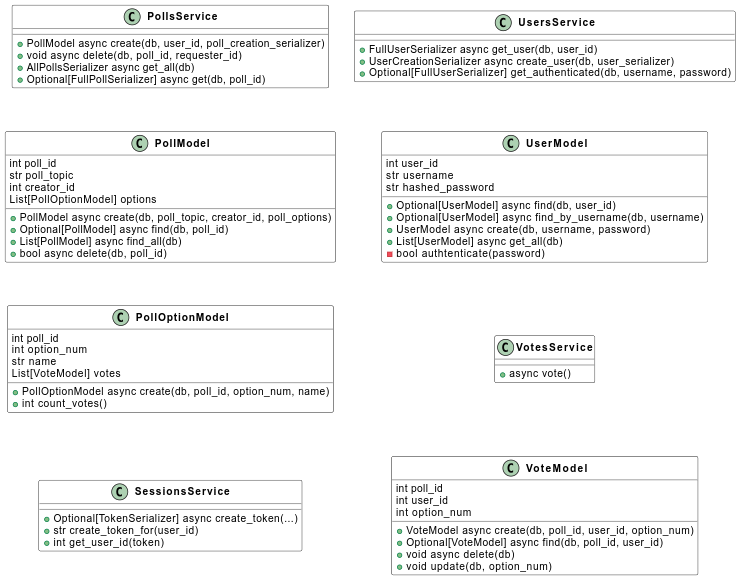
\includegraphics[width=\textwidth]{resources/http/python/class_diagram.png}
    \caption{Diagrama de clases de la implementación en Python del servidor HTTP de encuestas}
    \label{fig:http_python_class_diagram}
\end{figure}

En la Figura \ref{fig:http_python_class_diagram} se observan las clases principales del sistema, correspondientes a los \textit{Services} y \textit{Models}. Se omitieron los \textit{Serializers}, que carecen de lógica propia, pues Pydantic se encarga de ello. Los controllers se implementaron mediante funciones, siguiendo los patrones de diseño que FastAPI presenta en su documentación. En el Código \ref{code:http_python_endpoint} se muestra, a modo de ejemplo, la definición de uno de los endpoints. Es destacable la simplicidad del código: el boilerplate es muy poco, casi inexistente.

\begin{listing}
\begin{minted}[bgcolor=bg, breaklines]{python}
@router.get("/api/polls/{poll_id}", response_model=FullPollSerializer)
async def get_poll(poll_id: int, db: DbDependency):
    poll = await polls_service.get(db, poll_id)
    if not poll:
        raise HTTPException(status_code=404, detail="Poll not found")
    return poll
\end{minted}
\caption{Definición del endpoint GET /api/polls/\{poll\_id\} en Python, utilizando FastAPI}
\label{code:http_python_endpoint}
\end{listing}






\subsubsection{Ruby}

Ruby on Rails es, sin lugar a dudas, el framework más popular para realizar aplicaciones en Ruby\footnote{\url{https://github.com/EvanLi/Github-Ranking/blob/master/Top100/Ruby.md}}. % FIXME: not finished

\subsubsection{JavaScript}

Se eligió el lenguaje junto con la librería expressjs por ser uno de los más populares para el desarrollo de servidores y ser muy utilizado en la industria.
Se utilizaron las librerías: Typescript, para incluir tipado al lenguaje. Zod para validar los esquemas de datos en las rutas del servidor. Sequelize como ORM para interactuar con la base de datos.
El código se estructura principalmente en módulos de rutas, persistencia, middlewares y db.

\begin{listing}
\begin{minted}[bgcolor=bg, breaklines]{javascript}
pollsRouter.post("/polls", authenticateUser, validateNewPollParams, newPollHandler);
pollsRouter.get("/polls", getPollsHandler);

pollsRouter.get("/polls/:id", validatePollParams, getPollHandler);
pollsRouter.delete("/polls/:id", authenticateUser, validatePollParams, deletePollHandler);

pollsRouter.post("/polls/:poll_id/vote", authenticateUser, validateVoteParams, voteHandler);
\end{minted}
\caption{Definición de rutas en JS usando express}
\label{code:http_js_routes}
\end{listing}

\begin{listing}
\begin{minted}[bgcolor=bg, breaklines]{javascript}
export const authenticateUser = (
  req: Request,
  res: Response,
  next: NextFunction
) => {
  const auth = req.headers.authorization;

  if (!auth || typeof auth !== `string`)
    return next(createHttpError(401, "Missing Authorization Header"));

  const [type, jwt] = auth.split(" ");

  if (type !== "Bearer" || !jwt)
    return next(createHttpError(401, "Invalid Authorization Header"));

  const user: any = req.app.get("jwt").verify(jwt);
  const invalidUserId = !user?.id || typeof user.id != "number";
  const invalidUserName = !user.name || typeof user.name != "string";

  if (invalidUserId || invalidUserName)
    return next(createHttpError(401, "Invalid JWT"));

  getUser(user.name)
    .then((user) => {
      req.locals = { userId: user.id };
      next();
    })
    .catch(next);
};
\end{minted}
\caption{Middleware de autenticación de usuarios en JS}
\label{code:http_js_auth}
\end{listing}

Podemos ver en el Código \ref{code:http_js_routes} como se definen las rutas a partir de una composición de middlewares y controladores.
En el Código \ref{code:http_js_auth} podemos ver el middleware encargado de la autenticación de usuarios. La filosofia de express es que cada controlador sea mayormente independiente, compartiendo estado mediante las abstracciones de req y res. Estos controladores debes finalizar el manejo de la petición respondiendo o pasarla al siguiente controlador.

\subsubsection{Go}

Para Go se utilizó el framework Gin el cual permite crear un servidor http asincrónico. Además para la capa de persistencia se utilizó una base de datos postgres y se accedió a esta a través de la librería sql que es parte de la librería estándar de go. Se utilizó el mismo esquema de la base de datos que en los otros lenguajes y también se autenticó a los usuarios a través de de un token JWT para el cual se usó la librería golang-jwt. Además por comodidad se implementó la documentación con la librería gin-swagger la cual provee documentación bajo el estándar swagger para similar a lo que provee fastAPI.

\subsection{Métricas}

% FIXME

\subsection{Experiencias}

% FIXME

\subsection{Comparación}

El desarrollo con Java fue bastante directo, debido a que ya se tenía conocimiento del lenguaje al haberlo usado tanto en la facultad, como a nivel laboral. 

Al ser un lenguaje orientado a objetos, nos generó bastante boilerplate a pesar de que el proyecto era pequeño. En particular, configurar la parte de autenticación fue bastante engorroso. Al mismo tiempo, Spring nos “invita” a programar de cierta manera según su documentación oficial (separando en servicios, entidades y repositorios). Además, Spring se basa mucho en anotaciones para generar configuraciones, como por ejemplo, inyecciones de dependencias, determinar qué clases se ejecutan al levantar el proyecto, etc.

Al nivel de modelo de concurrencia, el modo “por defecto” de Spring (Java 17) utiliza un modelo sincrónico de 1 thread (del sistema operativo) por petición, partiendo de una threadpool con 200 threads de base. Si bien existe el modo asincrónico, no se tuvo en consideración para este desarrollo pero es algo para tener en cuenta para investigar.

En cuanto al nivel de configuración, resulta muy fácil pasar de una base de datos a otra. Por ejemplo, comenzamos desarrollando con una base en memoria (H2) y luego cambiamos a PostgreSQL con solo modificar la URL de conexión, sin modificar el código existente.

El manejo de errores viene dado principalmente por excepciones. Una vez que una excepción es lanzada, es atrapada por un controlador global de excepciones que nos permite devolver una respuesta personalizada en función de la excepción recibida.

\subsubsection{Go}

La experiencia de desarrollo en Go fue muy amena. Gin hace todo el trabajo pesado como el manejo de sockets y concurrencia y su interfaz es muy simple de usar. Una de las mejores cualidades de Gin es su manejo de los parámetros de la request como se ve en el el código 8.4.

\begin{listing}
\begin{minted}[bgcolor=bg, breaklines]{go}
var user models.UserInDB

if err := c.ShouldBindJSON(&user); err != nil {
	c.JSON(http.StatusBadRequest, gin.H{"error": "Invalid request body"})
	return
}
\end{minted}
\caption{Validación de request en Go}
\label{code:http_go}
\end{listing}

En este ejemplo tenemos el modelo de los datos de un usuario definidos en forma de un struct de go. Luego simplemente usamos la función \textit{ShouldBindJSON} con nuestra variable de usuario sobre el contexto y gin por su cuenta hace la validación de que la request tenga el formato correcto. Y de tener el formato correcto la variable se completa por sí sola. Además para el desarrollo fue muy útil gin-swagger, una biblioteca que nos permite generar documentación del estilo swagger para ir testeando los endpoints y detectar bugs de manera temprana.

Para la base de datos usamos un sistema postgres como en los otros ejemplos y para poder controlarla desde el código usamos la librería sql que es parte de la librería estándar de go. Esta librería fue una muy buena sorpresa ya que fue muy útil a la hora de interactuar con nuestra base de datos y todo esto sin agregar la complejidad que agrega una ORM al código.


\subsubsection{Java}

El desarrollo con Java fue bastante directo, debido a que ya se tenía conocimiento del lenguaje al haberlo usado tanto en la facultad, como a nivel laboral. 

Al ser un lenguaje orientado a objetos, nos generó bastante boilerplate a pesar de que el proyecto era pequeño. En particular, configurar la parte de autenticación fue bastante engorroso. Al mismo tiempo, Spring nos “invita” a programar de cierta manera según su documentación oficial (separando en servicios, entidades y repositorios). Además, Spring se basa mucho en anotaciones para generar configuraciones, como por ejemplo, inyecciones de dependencias, determinar qué clases se ejecutan al levantar el proyecto, etc.

Al nivel de modelo de concurrencia, el modo “por defecto” de Spring (Java 17) utiliza un modelo sincrónico de 1 thread (del sistema operativo) por petición, partiendo de una threadpool con 200 threads de base. Si bien existe el modo asincrónico, no se tuvo en consideración para este desarrollo pero es algo para tener en cuenta para investigar.

En cuanto al nivel de configuración, resulta muy fácil pasar de una base de datos a otra. Por ejemplo, comenzamos desarrollando con una base en memoria (H2) y luego cambiamos a PostgreSQL con solo modificar la URL de conexión, sin modificar el código existente.

El manejo de errores viene dado principalmente por excepciones. Una vez que una excepción es lanzada, es atrapada por un controlador global de excepciones que nos permite devolver una respuesta personalizada en función de la excepción recibida.



\subsubsection{Python}

FastAPI simplifica mucho la validación de datos de entrada y salida y es altamente configurable mediante la inyección de dependencias. Se destaca la generación automática de documentación (OpenAPI y Redoc) y la excelente integración con el IDE. Por otro lado, incluye un módulo de seguridad en el que se implementan un gran número de mecanismos de autenticación, entre ellos HTTP Basic, OAuth2 y API Keys.

SQLAlchemy implementa un ORM, aunque no es requerido para su uso. Dicho ORM es muy completo, implementa features avanzadas que otros ORM no: composite primary keys, mapeos autorreferenciales y cacheo de objetos, entre otras. Se puede utilizar de manera sincrónica o asincrónica.

Gracias a estas características del framework, el desarrollo fue bastante sencillo. La primera versión utilizaba métodos y funciones sincrónicas para interactuar con la base de datos. Posteriormente, esto se modificó para que sea asincrónico. El pasaje de una implementación a la otra no fue complejo, ya que tanto FastAPI como SQLAlchemy tienen soporte nativo para aplicaciones asincrónicas.


\subsubsection{Ruby}

Ruby on Rails basa su diseño en el principio “Convención sobre configuración”. El framework toma un gran número de decisiones a las que el programador debe adherir, entre las cuales se destacan las convenciones de nombres de las variables y la organización de los archivos de la aplicación. Esto trae dos consecuencias:
\begin{itemize}
    \item Un programador que ve un proyecto por primera vez puede familiarizarse rápidamente con el mismo, si ya tiene conocimiento en el framework
    \item El equipo de trabajo debe adaptarse al framework, y no al revés. Traducir una aplicación escrita en otro lenguaje (o incluso en otro framework de Ruby), resulta muy difícil
\end{itemize}

Al momento de crear un proyecto en Rails se incluyen un gran número de utilidades, tales como una base de datos (SQLite por defecto), un ORM, un sistema de migración de schemas, un archivo Dockerfile para poder ejecutar el servidor en un container, entre muchas otras cosas.

Una feature destacable es la consola, que permite, entre otras cosas, interactuar con la base de datos utilizando las clases definidas en el ORM. Es posible crear nuevos ítems, modificarlos o eliminarlos, lo cual es muy útil para probar funcionalidades nuevas sin tener que implementar los endpoints ni usar herramientas externas (como Postman o curl).

Todas estas características hicieron que el desarrollo sea muy particular. No fue sencillo, ya que el equipo no contaba con conocimientos previos ni de Ruby ni del framework. Sin embargo, creemos que tiene mucho mayor potencial para desarrollar una aplicación real y completa con relativa facilidad. Los frameworks utilizados en los otros lenguajes, si bien en principio son más fáciles de aprender, carecen de un ecosistema de bibliotecas propio. Ruby posee una gran cantidad de bibliotecas diseñadas para integrarse de manera armónica con un proyecto Rails, tales como Active Model Serializer\footnote{\url{https://github.com/rails-api/active_model_serializers}} y Bcrypt\footnote{\url{https://github.com/bcrypt-ruby/bcrypt-ruby}}.


\subsubsection{JavaScript}

El lenguaje es muy extensible y posee una gran cantidad de bibliotecas para las diferentes funcionalidades que pueden ser necesarios, esto tiene también su lado negativo, siendo que al tener mucha oferta puede dificultar elegir.
Dentro del stack seleccionado no se encontró una  manera efectiva de generar la documentación (swagger) de manera automática.
El ORM, Sequelize, no tiene soporte para asociaciones con clave primaria compuesta, con lo cual fue necesario realizar algunas peticiones en SQL crudo, por fuera del ORM.
La integración del lenguaje, y el tipado mediante Typescript, al IDE es muy buena, simplificando el desarrollo y la navegación del código.

\subsection{Conclusiones}

% FIXME

\section{Extensión del Trabajo}

En pos de facilitar la extensión del trabajo, se incluye esta sección dedicada a cómo se llevó a cabo la investigación y definición del trabajo y como podría ser extendido.

\subsection{Extensión siguiendo el desarrollo del Trabajo}

\subsubsection{Proceso de investigación y selección}

Nuestro flujo de trabajo se basó en la exploración independiente de casos de uso y lenguajes de programación que sean de interés para casos concurrentes.
Luego de eso se seleccionaron los casos de uso que consideramos más pertinentes y en base a esto se eligieron lenguajes de programación, teniendo en cuenta los investigados previamente así como aquellos que consideramos relevantes al caso.

\subsubsection{Agregando nuevos casos de uso}

Seleccionamos los casos de uso en base a aplicaciones de la vida real que utilizan o se pueden beneficiar de implementaciones concurrentes.

Realizamos una selección preliminar basándo nos en nuestra experiencia, recomendaciones e investigación, para luego generar un análisis más profundo de cada caso de uso a partir del cual seleccionamos los casos más pertinentes.

Algunos casos de uso que tuvimos en consideración pero no cubrimos:

\begin{itemize}
    \item Bases de Datos (descartado por su complejidad).
    \item IoT (descartado por necesidad de recursos).
    \item Aplicaciones en GPU (descartado por falta de lenguajes, monopolio de CUDA).
\end{itemize}

\subsubsection{Agregando nuevos lenguajes de programación}

Investigamos lenguajes de programación con características o predisposición a la concurrencia de manera independiente. Pero basamos su selección según los casos de uso:
Algunos de los factores a tener en cuenta para seleccionar lenguajes según un caso de uso son:

\begin{itemize}
    \item ¿Ya es utilizado para aplicaciones de estas características?
    \item ¿Hay proyectos con fin de utilizarlos para aplicaciones de estas características?
    \item ¿Provee alguna herramienta que pueda ser pertinente para este caso de uso?
    \item ¿Provee alguna herramienta o paradigma de concurrencia interesante?
    \item ¿El nivel de abstracción del lenguaje es acorde al caso de uso?
\end{itemize}

Algunos lenguajes que consideramos hubiera sido interesante cubrir:

\begin{itemize}
    \item Zig con Async (en desarrollo al tiempo de nuestra investigación)
    \item Python + Numba
    \item Clojure
    \item CUDA (no tiene competencia al tiempo de nuestra investigación)
\end{itemize}

\subsubsection{Re-enfoque sobre lo preexistente}

Durante el desarrollo tomamos ciertas decisiones que condicionan los casos de uso, la modificación de estas precondiciones podría generar resultados nuevos.

Con lo cual procedemos a listar algunas particularidades modificables según caso de uso:
\begin{itemize}
    \item Sistemas distribuidos
    \begin{itemize}
        \item Se hizo foco en middlewares brokerless.
        \item Se ignoró la tolerancia a fallas.
        \item Se seleccionaron sistemas de procesamiento de datos.
        \item Se seleccionaron casos que requieren mantener poco o nulo estado.
    \end{itemize}
    \item Criptografia
    \begin{itemize}
        \item Se seleccionó un algoritmo particular (podrían compararse otros).
        \item Se utilizó un paralelismo casi trivial.
        \item Se hizo procesamiento de información que no entra completamente en memoria.
    \end{itemize}
    \item Redes Neuronales
    \begin{itemize}
        \item Se utilizaron R.N. convolucionales (podrían compararse otros tipos).
        \item Se basó en clasificación de datos (podría tomarse otro caso de uso).
        \item Se evaluó el paralelismo en GPU.
        \item Dentro de la ciencia de datos, podrían evaluarse modelos que no utilicen R.N.
        \item Se entrenó en un solo computador, podría evaluarse de manera distribuida
        \item Se entrenó con relativamente pocos datos, podría evaluarse para big data
    \end{itemize}
\end{itemize}

\subsection{Extensión alternativa}

Cabe destacar que en nuestra investigación ponemos foco sobre los “casos de uso” y los “lenguajes” y sus frameworks, pero podría ser enriquecedor basarse en otros aspectos, por ejemplo:

\begin{itemize}
    \item Herramientas: comparar una misma herramienta en diferentes casos de uso. (e.g. zmq)
    \item Ambientes: comparar la portabilidad y desempeño en distintos ambientes.
    \item Foco en lenguajes primero: centrarse en los lenguajes y de ahí seleccionar casos de uso
    \item Resulta interesante pensar en lenguajes que podrían desplazar a C/C++ en algunos ámbitos, como Rust, Zig u otro\footnote{The Real C++ Killers: \url{https://hackernoon.com/the-real-c-killers-not-you-rust}}
    \item Foco en aspectos: buscar lenguajes en función de aspectos deseables (e.g. velocidad de desarrollo, concurrencia segura, extensibilidad)
\end{itemize}

\section{Referencias / Bibliografía}

\printbibliography %Prints bibliography

\section{Anexos} \label{annex} % FIXME: check that the values of the tables are ok

\subsection{\textit{Framework} de \textit{pipelines} distribuidos en exlixir} \label{sec:anex:elixir_pipelines}

\subsection{\textit{Profiling} y optimización de \textit{grids search} en exlixir} \label{sec:anex:elixir_gs_optimization}

\subsection{Métricas Extendidas}

\subsubsection{Grid Search}

\begin{table}[H]
\centering
\begin{tabular}{|l|c|c|c|}
\hline
\multicolumn{1}{|c|}{Measurement} & 4 Nodes & 8 Nodes & 16 Nodes \\ \hline
Worker Throughput & $1.42$ Results/Second & $1.28$ Results/Second & $1.26$ Results/Second \\ \hline
Combined Throughput & $1.60$ Results/Second & $18.2$ Results/Second & $34.8$ Results/Second \\ \hline
Work-time Variation & $0.83\%$& $0.25\%$& $0.38\%$\\ \hline
Memory Usage & $1.7-9.0$ MB/Worker & $1.6-9.0$ MB/Worker & $1.3-8.6$ MB/Worker \\ \hline
Network Usage (Tx) & 740 B/(s * Worker) & 710 B/(s * Worker) & 680 B/(s * Worker) \\ \hline
Network Usage (Rx) & 160 B/(s * Worker) & 155 B/(s * Worker) & 150 B/(s * Worker) \\ \hline
CPU Usage & 100\%/Worker & 100\%/Worker & 100\%/Worker \\ \hline
Completion Time & $41.5$ Minutes & $22.0$ Minutes & $11.2$ Minutes \\ \hline
\end{tabular}
\caption{C++ en FaMAF-2}
\end{table}

\begin{table}[H]
\centering
\begin{tabular}{|l|c|c|c|}
\hline
\multicolumn{1}{|c|}{Measurement} & 4 Nodes & 8 Nodes & 16 Nodes \\ \hline
Worker Throughput & $1.87$ Results/Second & $1.65$ Results/Second & $1.68$ Results/Second \\ \hline
Combined Throughput & $1.48$ Results/Second & $13.2$  Results/Second & $26.8$ Results/Second \\ \hline
Work-time Variation & 432\% & 705\% & $3.80\%$\\ \hline
Memory Usage & $1.29-4.00$ MB/Worker & $1.35-2.95$ MB/Worker & $1.00-4.50$ MB/Worker \\ \hline
Network Usage (Tx) & 580 B/(s * Worker) & 550 B/(s * Worker) & 600 B/(s * Worker) \\ \hline
Network Usage (Rx) & 130 B/(s * Worker) & 130 B/(s * Worker) & 132 B/(s * Worker) \\ \hline
CPU Usage & 100\%/Worker & 100\%/Worker & 100\%/Worker \\ \hline
Completion Time & $54.0$ Minutes & $26.7$ Minutes & $15.1$ Minutes \\ \hline
\end{tabular}
\caption{C++ en GCP}
\end{table}

\begin{table}[H]
\centering
\begin{tabular}{|l|c|c|c|}
\hline
\multicolumn{1}{|c|}{Measurement} & 4 Nodes & 8 Nodes & 16 Nodes \\ \hline
Worker Throughput & $1.64$ Results/Second & $1.63$ Results/Second & $1.6$ Results/Second \\ \hline
Combined Throughput & $1.57$ Results/Second & $1.85$ Results/Second & $1.47$ Results/Second \\ \hline
Work-time Variation & $1.57\%$& $1.95\%$& $1.83\%$\\ \hline
Memory Usage & 370 MB/Worker & 367 MB/Worker & 360 MB/Worker \\ \hline
Network Usage (Tx) & 352 B/(s * Worker) & 332 B/(s * Worker) & 322 B/(s * Worker) \\ \hline
Network Usage (Rx) & 195 B/(s * Worker) & 184 B/(s * Worker) & 179 B/(s * Worker) \\ \hline
CPU Usage & 100\%/Worker & 100\%/Worker & 100\%/Worker \\ \hline
Completion Time & 155 Minutes & 82.2Minutes & $42.1$ Minutes \\ \hline
\end{tabular}
\caption{Scala en FaMAF-2}
\end{table}

\begin{table}[H]
\centering
\begin{tabular}{|l|c|c|c|}
\hline
\multicolumn{1}{|c|}{Measurement} & 4 Nodes & 8 Nodes & 16 Nodes \\ \hline
Worker Throughput & $1.51$ Results/Second & $1.51$ Results/Second & $1.52$ Results/Second \\ \hline
Combined Throughput & $1.03$ Results/Second & $1.12$ Results/Second & $1.40$ Results/Second \\ \hline
Work-time Variation & $3.16\%$& $5.04\%$& $6.19\%$\\ \hline
Memory Usage & 52-64 MB/Worker & 52-60 MB/Worker & 52-58 MB/Worker \\ \hline
Network Usage (Tx) & 276 B/(s * Worker) & 281 B/(s * Worker) & 285 B/(s * Worker) \\ \hline
Network Usage (Rx) & 153 B/(s * Worker) & 156 B/(s * Worker) & 159 B/(s * Worker) \\ \hline
CPU Usage & 100\%/Worker & 100\%/Worker & 100\%/Worker \\ \hline
Completion Time & $196.8$ Minutes & $97.2$ Minutes & $47.7$ Minutes \\ \hline
\end{tabular}
\caption{Scala en GCP}
\end{table}

\begin{table}[H]
\centering
\begin{tabular}{|l|c|c|c|}
\hline
\multicolumn{1}{|c|}{Measurement} & 4 Nodes & 8 Nodes & 16 Nodes \\ \hline
Worker Throughput & $1.07$ Results/Second & $1.81$ Results/Second & $1.88$ Results/Second \\ \hline
Combined Throughput & $1.25$ Results/Second & $14.5$ Results/Second & $30.2$ Results/Second \\ \hline
Work-time Variation & 686\% & 466\% & 840\% \\ \hline
Memory Usage & $1.8-8.4$ MB/Worker & $1.1-8.7$ MB/Worker & $1.0-6.2$ MB/Worker \\ \hline
Network Usage (Tx) & 637 B/(s * Worker) & 598 B/(s * Worker) & 578 B/(s * Worker) \\ \hline
Network Usage (Rx) & 150 B/(s * Worker) & 130 B/(s * Worker) & 126 B/(s * Worker) \\ \hline
CPU Usage & 100\%/Worker & 100\%/Worker & 100\%/Worker \\ \hline
Completion Time & $49.9$ Minutes & $27.0$ Minutes & $13.4$ Minutes \\ \hline
\end{tabular}
\caption{Go en FaMAF-2}
\end{table}

\begin{table}[H]
\centering
\begin{tabular}{|l|c|c|c|}
\hline
\multicolumn{1}{|c|}{Measurement} & 4 Nodes & 8 Nodes & 16 Nodes \\ \hline
Worker Throughput & $1.52$ Results/Second & $1.54$ Results/Second & $1.51$ Results/Second \\ \hline
Combined Throughput & $1.91$ Results/Second & $11.7$ Results/Second & $23.5$ Results/Second \\ \hline
Work-time Variation & $1.275$ \% & $1.21$ \% & $1.644$ \% \\ \hline
Memory Usage & $1.4-4.8$ MB/Worker & $1.8-4.4$ MB/Worker & $1.4-2.8$ MB/Worker \\ \hline
Network Usage (Tx) & 462 B/(s * Worker) & 490 B/(s * Worker) & 480 B/(s * Worker) \\ \hline
Network Usage (Rx) & 102 B/(s * Worker) & 104 B/(s * Worker) & 100 B/(s * Worker) \\ \hline
CPU Usage & 100\%/Worker & 100\%/Worker & 100\%/Worker \\ \hline
Completion Time & $67.2$ Minutes & $34.2$ Minutes & $17.2$ Minutes \\ \hline
\end{tabular}
\caption{Go en GCP}
\end{table}

\begin{table}[H]
\centering
\begin{tabular}{|l|c|c|c|}
\hline
\multicolumn{1}{|c|}{Measurement} & 4 Nodes & 8 Nodes & 16 Nodes \\ \hline
Worker Throughput & $1.36$ Results/Second & $1.26$ Results/Second & $1.26$ Results/Second \\ \hline
Combined Throughput & $1.43$ Results/Second & $10.1$ Results/Second & $20.0$ Results/Second \\ \hline
Work-time Variation & $1.83\%$& $1.21\%$& 757\% \\ \hline
Memory Usage & $1.24$ GB/Worker & $1.24$ GB/Worker & $1.18$ MB/Worker \\ \hline
Network Usage (Tx) & 327 B/(s * Worker) & 305 B/(s * Worker) & 302 B/(s * Worker) \\ \hline
Network Usage (Rx) & 220 B/(s * Worker) & 207 B/(s * Worker) & 206 B/(s * Worker) \\ \hline
CPU Usage & 100\%/Worker & 100\%/Worker & 100\%/Worker \\ \hline
Completion Time & $73.2$ Minutes & $39.2$ Minutes & $20.0$ Minutes \\ \hline
\end{tabular}
\caption{Julia en FaMAF-2}
\end{table}

\begin{table}[H]
\centering
\begin{tabular}{|l|c|c|c|}
\hline
\multicolumn{1}{|c|}{Measurement} & 4 Nodes & 8 Nodes & 16 Nodes \\ \hline
Worker Throughput & $1.18$ Results/Second & $1.16$ Results/Second & $1.18$ Results/Second \\ \hline
Combined Throughput & $1.69$ Results/Second & $1.19$ Results/Second & $18.8$ Results/Second \\ \hline
Work-time Variation & $2.40\%$& $1.58\%$& $2.19\%$\\ \hline
Memory Usage & $1.10$ GB/Worker & $1.08$ GB/Worker & $1.09$ GB/Worker \\ \hline
Network Usage (Tx) & 280 B/(s * Worker) & 276 B/(s * Worker) & 282 B/(s * Worker) \\ \hline
Network Usage (Rx) & 189 B/(s * Worker) & 187 B/(s * Worker) & 194 B/(s * Worker) \\ \hline
CPU Usage & 100\%/Worker & 100\%/Worker & 100\%/Worker \\ \hline
Completion Time & $85.2$ Minutes & $43.3$ Minutes & $21.3$ Minutes \\ \hline
\end{tabular}
\caption{Julia en GCP}
\end{table}

\begin{table}[H]
\centering
\begin{tabular}{|l|c|c|c|}
\hline
\multicolumn{1}{|c|}{Measurement} & 4 Nodes & 8 Nodes & 16 Nodes \\ \hline
Worker Throughput & $1.25$ Results/Second & $1.24$ Results/Second & $1.23$ Results/Second \\ \hline
Combined Throughput & $1.991$ Results/Second & $1.90$ Results/Second & $1.74$ Results/Second \\ \hline
Work-time Variation & $3.05\%$& 659\% & $2.37\%$\\ \hline
Memory Usage & 83-95 MB/Worker & 84-96 MB/Worker & 84 MB/Worker \\ \hline
Network Usage (Tx) & 376 B/(s * Worker) & 399 B/(s * Worker) & 469 B/(s * Worker) \\ \hline
Network Usage (Rx) & 266 B/(s * Worker) & 296 B/(s * Worker) & 367 B/(s * Worker) \\ \hline
CPU Usage & 100\%/Worker & 100\%/Worker & 100\%/Worker \\ \hline
Completion Time & $403.2$ Minutes & $209.4$ Minutes & $106.8$ Minutes \\ \hline
\end{tabular}
\caption{Elixir en FaMAF-2}
\end{table}

\begin{table}[H]
\centering
\begin{tabular}{|l|c|c|c|c|c|}
\hline
\multicolumn{1}{|c|}{Measurement} & C++ & Scala & Go & Julia & Elixir \\ \hline
\begin{tabular}[c]{@{}l@{}}Combined Throughput\\ {[}Results/Second{]}\end{tabular} & $18.2$ & $4.85$ & $14.5$ & $10.1$ & $1.90$ \\ \hline
Work-time Variation {[}\%{]} & $0.25$ & $1.95$ & $0.466$ & $1.21$ & $0.659$ \\ \hline
Memory Usage {[}MB/Worker{]} & $1.6-9.0$ & 367 & $4.1-8.7$ & $1240$ & 84-96 \\ \hline
\begin{tabular}[c]{@{}l@{}}Network Usage (Tx)\\ {[}B/(s * Worker){]}\end{tabular} & 710 & 332 & 598 & 305 & 399 \\ \hline
\begin{tabular}[c]{@{}l@{}}Network Usage (Rx)\\ {[}B/(s * Worker){]}\end{tabular} & 155 & 184 & 130 & 207 & 296 \\ \hline
Completion Time {[}Minutes{]} & $22.0$ & $82.2$ & $27.0$ & $39.2$ & $209.4$ \\ \hline
\end{tabular}
\caption{Resumen de 8 Workers en FaMAF-2}
\label{tab:gs:8_workers_famaf2}
\end{table}

\begin{table}[H]
\centering
\begin{tabular}{|l|c|c|c|c|c|}
\hline
\multicolumn{1}{|c|}{Measurement} & C++ & Scala & Go & Julia & Elixir \\ \hline
\begin{tabular}[c]{@{}l@{}}Combined Throughput\\ {[}Results/Second{]}\end{tabular} & $13.2$ & $4.12$ & $11.7$ & $9.19$ & - \\ \hline
Work-time Variation {[}\%{]} & $0.705$ & $5.04$ & $5.21$ & $1.58$ & - \\ \hline
Memory Usage {[}MB/Worker{]} & $1.35-2.95$ & 52-60 & $1.8-4.4$ & 1080 & - \\ \hline
\begin{tabular}[c]{@{}l@{}}Network Usage (Tx)\\ {[}B/(s * Worker{]}\end{tabular} & 550 & 281 & 490 & 276 & - \\ \hline
\begin{tabular}[c]{@{}l@{}}Network Usage (Rx)\\ {[}B/(s * Worker){]}\end{tabular} & 130 & 156 & 104 & 187 & - \\ \hline
Completion Time {[}Minutes{]} & $26.7$ & $97.2$ & $34.2$ & $43.3$ & - \\ \hline
\end{tabular}
\caption{Resumen de 8 Workers en GCP}
\end{table}

\begin{table}[H]
\centering
\begin{tabular}{|ccc|}
\hline
\multicolumn{3}{|c|}{Grid Search - Container Size} \\ \hline
\multicolumn{1}{|c|}{\multirow{2}{*}{C++}} & \multicolumn{1}{c|}{Manager} & $17.4$ MB \\ \cline{2-3} 
\multicolumn{1}{|c|}{} & \multicolumn{1}{c|}{Worker} & $17.3$ MB \\ \hline
\multicolumn{1}{|c|}{\multirow{3}{*}{Scala}} & \multicolumn{1}{c|}{Manager} & 192 MB \\ \cline{2-3} 
\multicolumn{1}{|c|}{} & \multicolumn{1}{c|}{Worker} & 192 MB \\ \cline{2-3} 
\multicolumn{1}{|c|}{} & \multicolumn{1}{c|}{Middleware} & 180 MB \\ \hline
\multicolumn{1}{|c|}{\multirow{3}{*}{Go}} & \multicolumn{1}{c|}{Manager} & $15.5$ MB \\ \cline{2-3} 
\multicolumn{1}{|c|}{} & \multicolumn{1}{c|}{Worker} & $15.4$ MB \\ \cline{2-3} 
\multicolumn{1}{|c|}{} & \multicolumn{1}{c|}{Middleware} & $14.4$ MB \\ \hline
\multicolumn{1}{|c|}{\multirow{2}{*}{Julia}} & \multicolumn{1}{c|}{Manager} & 754 MB \\ \cline{2-3} 
\multicolumn{1}{|c|}{} & \multicolumn{1}{c|}{Worker} & 795 MB \\ \hline
\multicolumn{1}{|c|}{\multirow{2}{*}{Elixir}} & \multicolumn{1}{c|}{Manager} & \textgreater{}84.8MB \\ \cline{2-3} 
\multicolumn{1}{|c|}{} & \multicolumn{1}{c|}{Worker} & \textgreater{}84.8MB \\ \hline
\end{tabular}
\caption{Tamaño de Containers}
\end{table}

\subsubsection{Procesamiento de Imágenes}

\begin{table}[H]
\centering
\begin{tabular}{|l|l|l|l|}
\hline
\multicolumn{1}{|c|}{Measurement} & \multicolumn{1}{c|}{2 Nodes} & \multicolumn{1}{c|}{4 Nodes} & \multicolumn{1}{c|}{6 Nodes} \\ \hline
Combined Throughput & 172 Results/Second & 250 Results/Second & \multicolumn{1}{c|}{263 Results/Second} \\ \hline
Max Work-time Variation & $5.5\%$& $2.8\%$& $5.6\%$\\ \hline
Max Memory Usage & 70 MB/Worker & 55 MB/Worker & 41 MB/Worker \\ \hline
Max Network Usage (Tx) & 32 KB/(s * Worker) & 22 KB/(s * Worker) & 14 B/(s * Worker) \\ \hline
Max Network Usage (Rx) & 18 KB/(s * Worker) & 12 KB/(s * Worker) & $1.2$ B/(s * Worker) \\ \hline
CPU Usage - Format & 100\%/Worker & 75 \%/Worker & 50 \%/Worker \\ \hline
CPU Usage - Resolution & 56\% / Worker & 40 \%/Worker & 35 \%/Worker \\ \hline
CPU Usage - Size & 18\%/Worker & 10 \%/Worker & 10\%/Worker \\ \hline
Completion Time & $26.1$ Minutes & $18.0$ Minutes & $17.1$ Minutes \\ \hline
\end{tabular}
\caption{C++ en FaMAF-2}
\end{table}

\begin{table}[H]
\centering
\begin{tabular}{|l|l|l|l|}
\hline
\multicolumn{1}{|c|}{Measurement} & \multicolumn{1}{c|}{2 Nodes} & \multicolumn{1}{c|}{4 Nodes} & \multicolumn{1}{c|}{6 Nodes} \\ \hline
Combined Throughput & $75.2$ Results/Second & 84 Results/Second & 119 Results/Second \\ \hline
Max Work-time Variation & $1.1$ \% & $1.9$ \% & $1.3$ \% \\ \hline
Max Memory Usage & 180 MB/Worker & 97 MB/Worker & 75 MB/Worker \\ \hline
Max Network Usage (Tx) & 13 KB/(s * Worker) & $1.9$ KB/(s * Worker) & $1.8$ KB/(s * Worker) \\ \hline
Max Network Usage (Rx) & $1.2$ KB/(s * Worker) & $1.8$ KB/(s * Worker) & $1.8$ KB/(s * Worker) \\ \hline
CPU Usage - Format & 60 \%/Worker & 35\%/Worker & 35\%/Worker \\ \hline
CPU Usage - Resolution & 22 \%/Worker & 10 \%/Worker & 12 \%/Worker \\ \hline
CPU Usage - Size & 7 \%/Worker & 5 \%/Worker & 5 \%/Worker \\ \hline
Completion Time & $19.9$ Minutes & $17.8$ Minutes & $12.6$ Minutes \\ \hline
\end{tabular}
\caption{C++ en GCP}
\end{table}

\begin{table}[H]
\centering
\begin{tabular}{|l|l|l|l|}
\hline
\multicolumn{1}{|c|}{Measurement} & \multicolumn{1}{c|}{2 Nodes} & \multicolumn{1}{c|}{4 Nodes} & \multicolumn{1}{c|}{6 Nodes} \\ \hline
Combined Throughput & 117 Results/Second & 139 Results/Second & 162 Results/Second \\ \hline
Max Work-time Variation & $0.8\%$& $3.2\%$& $2.7\%$\\ \hline
Max Memory Usage & 830 MB/Worker & 715 MB/Worker & 660 MB/Worker \\ \hline
Max Network Usage (Tx) & 24 KB/(s * Worker) & 15 KB/(s * Worker) & 12 KB/(s * Worker) \\ \hline
Max Network Usage (Rx) & 18 KB/(s * Worker) & 11 KB/(s * Worker) & $1.9$ KB/(s * Worker) \\ \hline
CPU Usage - Format & 85 \%/Worker & 55 \%/Worker & 41 \%/Worker \\ \hline
CPU Usage - Resolution & 65 \%/Worker & 38 \%/Worker & 30 \%/Worker \\ \hline
CPU Usage - Size & 19 \%/Worker & 10 \%/Worker & 8 \%/Worker \\ \hline
Completion Time & $38.4$ Minutes & $32.3$ Minutes & $27.7$ Minutes \\ \hline
\end{tabular}
\caption{Scala en FaMAF-2}
\end{table}

\begin{table}[H]
\centering
\begin{tabular}{|l|l|l|l|}
\hline
\multicolumn{1}{|c|}{Measurement} & \multicolumn{1}{c|}{2 Nodes} & \multicolumn{1}{c|}{4 Nodes} & \multicolumn{1}{c|}{6 Nodes} \\ \hline
Combined Throughput & $75.3$ Results/Second & 109 Results/Second & 153 Results/Second \\ \hline
Max Work-time Variation & $1.3$ \% & $1.4$ \% & $1.6$ \% \\ \hline
Max Memory Usage & 330 MB/Worker & 240 MB/Worker & 200MB/Worker \\ \hline
Max Network Usage (Tx) & 15 KB/(s * Worker) & 12 KB/(s * Worker) & 11 KB/(s * Worker) \\ \hline
Max Network Usage (Rx) & 11 KB/(s * Worker) & $1.4$ KB/(s * Worker) & $1.0$ KB/(s * Worker) \\ \hline
CPU Usage - Format & 64 \%/Worker & 44 \%/Worker & 42 \%/Worker \\ \hline
CPU Usage - Resolution & 37 \%/Worker & 28 \%/Worker & 27 \%/Worker \\ \hline
CPU Usage - Size & 13 \%/Worker & 8 \%/Worker & 9 \%/Worker \\ \hline
Completion Time & $19.9$ Minutes & $13.7$ Minutes & $1.8$ Minutes \\ \hline
\end{tabular}
\caption{Scala en GCP}
\end{table}

\begin{table}[H]
\centering
\begin{tabular}{|l|l|l|l|}
\hline
\multicolumn{1}{|c|}{Measurement} & \multicolumn{1}{c|}{2 Nodes} & \multicolumn{1}{c|}{4 Nodes} & \multicolumn{1}{c|}{6 Nodes} \\ \hline
Combined Throughput & 50 Results/Second & 92 Results/Second & 135 Results/Second \\ \hline
Max Work-time Variation & $2.11\%$& $5.78\%$& $1.42$ \% \\ \hline
Max Memory Usage & 128 MB/Worker & 96 MB/Worker & 68 MB/Worker \\ \hline
Max Network Usage (Tx) & $1.85$ KB/(s * Worker) & $1.21$ KB/(s * Worker) & $1.03$ KB/(s * Worker) \\ \hline
Max Network Usage (Rx) & $1.51$ KB/(s * Worker) & $1.23$ KB/(s * Worker) & $1.16$ KB/(s * Worker) \\ \hline
CPU Usage - Format & 100\%/Worker & 100\%/Worker & 100\%/Worker \\ \hline
CPU Usage - Resolution & 80\%/Worker & 80\%/Worker & 80\%/Worker \\ \hline
CPU Usage - Size & 20\%/Worker & 20\%/Worker & 20\%/Worker \\ \hline
Completion Time & $89.9$ Minutes & $48.8$ Minutes & $33.3$ Minutes \\ \hline
\end{tabular}
\caption{Go en FaMAF-2}
\end{table}

\begin{table}[H]
\centering
\begin{tabular}{|l|l|l|l|}
\hline
\multicolumn{1}{|c|}{Measurement} & \multicolumn{1}{c|}{2 Nodes} & \multicolumn{1}{c|}{4 Nodes} & \multicolumn{1}{c|}{6 Nodes} \\ \hline
Combined Throughput & 40 Results/Second & 75 Results/Second & 104 Results/Second \\ \hline
Max Work-time Variation & $1.96$ \% & $11.3$ \% & $24.9$ \% \\ \hline
Max Memory Usage & 144 MB/Worker & 90 MB/Worker & 64 MB/Worker \\ \hline
Max Network Usage (Tx) & $1.03$ KB/(s * Worker) & $1.62$ KB/(s * Worker) & $1.20$ KB/(s * Worker) \\ \hline
Max Network Usage (Rx) & $1.58$ KB/(s * Worker) & $1.37$ KB/(s * Worker) & $1.12$ KB/(s * Worker) \\ \hline
CPU Usage - Format & 80\%/Worker & 80\%/Worker & 80\%/Worker \\ \hline
CPU Usage - Resolution & 30\%/Worker & 30\%/Worker & 25\%/Worker \\ \hline
CPU Usage - Size & 5\%/Worker & 5\%/Worker & 5\%/Worker \\ \hline
Completion Time & $37.5$ Minutes & $20.0$ Minutes & $14.4$ Minutes \\ \hline
\end{tabular}
\caption{Go en GCP}
\end{table}

\begin{table}[H]
\centering
\begin{tabular}{|l|l|l|l|}
\hline
\multicolumn{1}{|c|}{Measurement} & \multicolumn{1}{c|}{2 Nodes} & \multicolumn{1}{c|}{4 Nodes} & \multicolumn{1}{c|}{6 Nodes} \\ \hline
Combined Throughput & 400 Results/Second & 745 Results/Second & 1.1K Results/Second \\ \hline
Max Work-time Variation & $1.7$ \% & $1.5$ \% & 8 \% \\ \hline
Max Memory Usage & 448 MB/Worker & 460 MB/Worker & 450 MB/Worker \\ \hline
Max Network Usage (Tx) & 136 KB/(s * Worker) & 125 KB/(s * Worker) & 118 KB/(s * Worker) \\ \hline
Max Network Usage (Rx) & 55 KB/(s * Worker) & 50 KB/(s * Worker) & 48 KB/(s * Worker) \\ \hline
CPU Usage - Format & 92\%/Worker & 96\%/Worker & 96\%/Worker \\ \hline
CPU Usage - Resolution & 73\%/Worker & 69 \%/Worker & 72 \%/Worker \\ \hline
CPU Usage - Size & 34 \%/Worker & 31\%/Worker & 30 \%/Worker \\ \hline
Completion Time & $11.2$ Minutes & $1.0$ Minutes & $1.1$ Minutes \\ \hline
\end{tabular}
\caption{Julia en FaMAF-2}
\end{table}

\begin{table}[H]
\centering
\begin{tabular}{|l|l|l|l|}
\hline
\multicolumn{1}{|c|}{Measurement} & \multicolumn{1}{c|}{2 Nodes} & \multicolumn{1}{c|}{4 Nodes} & \multicolumn{1}{c|}{6 Nodes} \\ \hline
Combined Throughput & $82.6$ Results/Second & 215 Results/Second & 235 Results/Second \\ \hline
Max Work-time Variation & $1.5$ \% & $1.7$ \% & $1.3$ \% \\ \hline
Max Memory Usage & $1.13$ GB/Worker & 896 MB/Worker & 704 MB/Worker \\ \hline
Max Network Usage (Tx) & 28 KB/(s * Worker) & 37 KB/(s * Worker) & 27 KB/(s * Worker) \\ \hline
Max Network Usage (Rx) & 11 KB/(s * Worker) & 15 KB/(s * Worker) & 11 KB/(s * Worker) \\ \hline
CPU Usage - Format & 24\%/Worker & 38\%/Worker & 25\%/Worker \\ \hline
CPU Usage - Resolution & 18\%/Worker & 24\%/Worker & 19\%/Worker \\ \hline
CPU Usage - Size & 9\%/Worker & 11\%/Worker & 7\%/Worker \\ \hline
Completion Time & $18.1$ Minutes & $1.9$ Minutes & $1.37$ Minutes \\ \hline
\end{tabular}
\caption{Julia en GCP}
\end{table}

\begin{table}[H]
\centering
\begin{tabular}{|l|l|l|l|}
\hline
\multicolumn{1}{|c|}{Measurement} & \multicolumn{1}{c|}{2 Nodes} & \multicolumn{1}{c|}{4 Nodes} & \multicolumn{1}{c|}{6 Nodes} \\ \hline
Combined Throughput & $78.2$ Results/Second & 141 Results/Second & 245 Results/Second \\ \hline
Max Work-time Variation & $1.3$ \% & $1.3$ \% & $1.0$ \% \\ \hline
Max Memory Usage & 140 MB/Worker & 115 MB/Worker & 650 MB/Worker \\ \hline
Max Network Usage (Tx) & $1.2$ KB/(s * Worker) & $1.2$ KB/(s * Worker) & $1.4$ KB/(s * Worker) \\ \hline
Max Network Usage (Rx) & $1.4$ KB/(s * Worker) & $1.0$ KB/(s * Worker) & $1.6$ KB/(s * Worker) \\ \hline
CPU Usage - Format & 96 \%/Worker & 77 \%/Worker & 77 \%/Worker \\ \hline
CPU Usage - Resolution & 110 \%/Worker & 93 \%/Worker & 92 \%/Worker \\ \hline
CPU Usage - Size & 33 \%/Worker & 25 \%/Worker & 26 \%/Worker \\ \hline
Completion Time & $57.5$ Minutes & $31.9$ Minutes & $18.3$ Minutes \\ \hline
\end{tabular}
\caption{Elixir en FaMAF-2}
\end{table}

\begin{table}[H]
\centering
\begin{tabular}{|l|l|l|l|}
\hline
\multicolumn{1}{|c|}{Measurement} & \multicolumn{1}{c|}{2 Nodes} & \multicolumn{1}{c|}{4 Nodes} & \multicolumn{1}{c|}{6 Nodes} \\ \hline
Combined Throughput & $57.6$ Results/Second & $85.1$ Results/Second & 103 Results/Second \\ \hline
Max Work-time Variation & $1.6$ \% & $1.6$ \% & $1.6$ \% \\ \hline
Max Memory Usage & 390 MB/Worker & 240 MB/Worker & 180 MB/Worker \\ \hline
Max Network Usage (Tx) & $1.6$ KB/(s * Worker) & $1.8$ KB/(s * Worker) & $1.0$ KB/(s * Worker) \\ \hline
Max Network Usage (Rx) & $1.3$ KB/(s * Worker) & $1.8$ KB/(s * Worker) & $1.5$ KB/(s * Worker) \\ \hline
CPU Usage - Format & 44 \%/Worker & 35 \%/Worker & 28 \%/Worker \\ \hline
CPU Usage - Resolution & 26 \%/Worker & 20 \%/Worker & 18 \%/Worker \\ \hline
CPU Usage - Size & 18 \%/Worker & 16 \%/Worker & 12 \%/Worker \\ \hline
Completion Time & $26.0$ Minutes & $17.6$ Minutes & $14.54$ Minutes \\ \hline
\end{tabular}
\caption{Elixir en GCP}
\end{table}

\begin{table}[H]
\centering
\begin{tabular}{|l|c|c|c|c|c|}
\hline
\multicolumn{1}{|c|}{\textbf{Measurement}} & \textbf{C++} & \textbf{Scala} & \textbf{Go} & \textbf{Julia} & \textbf{Elixir} \\ \hline
\begin{tabular}[c]{@{}l@{}}Combined Throughput\\ {[}Results/Second{]}\end{tabular} & 250 & 139 & 92 & 745 & 141 \\ \hline
Max Work-time Variation {[}\%{]} & $1.8$ & $1.2$ & $1.78$ & $1.5$ & $1.3$ \\ \hline
Max Memory Usage {[}MB/Worker{]} & 55 & 715 & 96 & 460 & 115 \\ \hline
\begin{tabular}[c]{@{}l@{}}Max Network Usage (Tx)\\ {[}KB/(s * Worker){]}\end{tabular} & 22 & 15 & $1.21$ & 125 & $1.2$ \\ \hline
\begin{tabular}[c]{@{}l@{}}Max Network Usage (Rx)\\ {[}KB/(s * Worker){]}\end{tabular} & 12 & 11 & $1.23$ & 50 & $1.0$ \\ \hline
CPU Usage - Format {[}\%/Worker{]} & 75 & 55 & 100 & 96 & 77 \\ \hline
CPU Usage - Resolution {[}\%/Worker{]} & 40 & 38 & 80 & 69 & 93 \\ \hline
CPU Usage - Size {[}\%/Worker{]} & 10 & 10 & 20 & 31 & 25 \\ \hline
Completion Time {[}Minutes{]} & $18.0$ & $32.3$ & $48.8$ & $1.0$ & $17.4$ \\ \hline
\end{tabular}
\caption{Resumen de 4 Nodos en FaMAF-2}
\label{tab:ip:4_workers_famaf_2}
\end{table}

\begin{table}[H]
\centering
\begin{tabular}{|l|c|c|c|c|c|}
\hline
\multicolumn{1}{|c|}{\textbf{Measurement}} & \textbf{C++} & \textbf{Scala} & \textbf{Go} & \textbf{Julia} & \textbf{Elixir} \\ \hline
\begin{tabular}[c]{@{}l@{}}Combined Throughput\\ {[}Results/Second{]}\end{tabular} & 84 & 109 & 75 & 215 & $85.1$ \\ \hline
Max Work-time Variation {[}\%{]} & $1.9$ & $1.4$ & $11.3$ & $1.7$ & $1.6$ \\ \hline
Max Memory Usage {[}MB/Worker{]} & 97 & 240 & 90 & 896 & 240 \\ \hline
\begin{tabular}[c]{@{}l@{}}Max Network Usage (Tx)\\ {[}KB/(s * Worker){]}\end{tabular} & $1.9$ & 12 & $1.62$ & 37 & $1.8$ \\ \hline
\begin{tabular}[c]{@{}l@{}}Max Network Usage (Rx)\\ {[}KB/(s * Worker){]}\end{tabular} & $1.8$ & $1.4$ & $1.37$ & 15 & $1.8$ \\ \hline
CPU Usage - Format {[}\%/Worker{]} & 35 & 44 & 80 & 38 & 35 \\ \hline
CPU Usage - Resolution {[}\%/Worker{]} & 10 & 28 & 30 & 24 & 20 \\ \hline
CPU Usage - Size {[}\%/Worker{]} & 5 & 8 & 5 & 11 & 16 \\ \hline
Completion Time {[}Minutes{]} & $17.8$ & $13.7$ & $20.0$ & $1.9$ & $17.6$ \\ \hline
\end{tabular}
\caption{Resumen de 4 Nodos en GCP}
\end{table}

\begin{table}[H]
\centering
\begin{tabular}{|ccc|}
\hline
\multicolumn{3}{|c|}{Image Processing - Container Size} \\ \hline
\multicolumn{1}{|c|}{\multirow{3}{*}{C++}} & \multicolumn{1}{c|}{Manager} & $1.45$ GB \\ \cline{2-3} 
\multicolumn{1}{|c|}{} & \multicolumn{1}{c|}{Worker} & $1.45$ GB \\ \cline{2-3} 
\multicolumn{1}{|c|}{} & \multicolumn{1}{c|}{Middleware} & $1.45$ GB \\ \hline
\multicolumn{1}{|c|}{\multirow{3}{*}{Scala}} & \multicolumn{1}{c|}{Manager} & 194 MB \\ \cline{2-3} 
\multicolumn{1}{|c|}{} & \multicolumn{1}{c|}{Worker} & 194 MB \\ \cline{2-3} 
\multicolumn{1}{|c|}{} & \multicolumn{1}{c|}{Middleware} & 180 MB \\ \hline
\multicolumn{1}{|c|}{\multirow{3}{*}{Go}} & \multicolumn{1}{c|}{Manager} & 15 MB \\ \cline{2-3} 
\multicolumn{1}{|c|}{} & \multicolumn{1}{c|}{Worker} & $15.8$ MB \\ \cline{2-3} 
\multicolumn{1}{|c|}{} & \multicolumn{1}{c|}{Middleware} & $14.4$ MB \\ \hline
\multicolumn{1}{|c|}{\multirow{2}{*}{Julia}} & \multicolumn{1}{c|}{Manager} & $1.96$ GB \\ \cline{2-3} 
\multicolumn{1}{|c|}{} & \multicolumn{1}{c|}{Worker} & $1.96$ GB \\ \hline
\multicolumn{1}{|c|}{\multirow{2}{*}{Elixir}} & \multicolumn{1}{c|}{Manager} & \textgreater{}$84.8$ MB \\ \cline{2-3} 
\multicolumn{1}{|c|}{} & \multicolumn{1}{c|}{Worker} & \textgreater{}$84.8$ MB \\ \hline
\end{tabular}
\caption{Tamaño de Containers}
\end{table}

\subsubsection{Criptografía: AES}

\begin{table}[H]
\centering
\begin{tabular}{|c|c|c|c|c|c|}
\hline
Metrica & Rust & Go & Julia & Scala & Zig \\ \hline
Duration (Min) & $16.9$ & 102 & $15.9$ & 252 & $24.3$ \\ \hline
Memory Usage (MB) & 231 & $15.9$ & 548 & 566 & $1.27$ \\ \hline
CPU Usage & 300\% & 337\% & 229\% & 179\% & 232\% \\ \hline
\end{tabular}
\caption{Resumen de corridas en FaMAF-2}
\end{table}

\subsubsection{Redes neuronales: Regresión}

\begin{table}[H]
\centering
\begin{tabular}{|c|c|c|c|c|}
\hline
& \multicolumn{2}{c|}{Python} & \multicolumn{2}{c|}{Julia} \\ \hline
Metrica & Tensorflow/Keras & PyTorch & Flux & SciKitLearn \\ \hline
Duration (Min) & 21 & $1.3$ & $1.56$ & $1.35$ \\ \hline
Memory Usage (GB) & $1.55$ & $1.16$ & $1.69$ & $1.33$ \\ \hline
CPU Usage & $126.00\%$ & $99.99\%$& $106.00\%$& $105.00\%$\\ \hline
GPU Usage (GB) & $1.76$ & $1.08$ & $1.69$ & - \\ \hline
RMSE & $50500$ & $52582$ & $53400$ & $49000$ \\ \hline
\end{tabular}
\caption{Resumen de corridas en FaMAF-2}
\label{tab:my-table}
\end{table}

\end{document}
